\documentclass[twoside]{book}

% Packages required by doxygen
\usepackage{fixltx2e}
\usepackage{calc}
\usepackage{doxygen}
\usepackage[export]{adjustbox} % also loads graphicx
\usepackage{graphicx}
\usepackage[utf8]{inputenc}
\usepackage{makeidx}
\usepackage{multicol}
\usepackage{multirow}
\PassOptionsToPackage{warn}{textcomp}
\usepackage{textcomp}
\usepackage[nointegrals]{wasysym}
\usepackage[table]{xcolor}

% Font selection
\usepackage[T1]{fontenc}
\usepackage[scaled=.90]{helvet}
\usepackage{courier}
\usepackage{amssymb}
\usepackage{sectsty}
\renewcommand{\familydefault}{\sfdefault}
\allsectionsfont{%
  \fontseries{bc}\selectfont%
  \color{darkgray}%
}
\renewcommand{\DoxyLabelFont}{%
  \fontseries{bc}\selectfont%
  \color{darkgray}%
}
\newcommand{\+}{\discretionary{\mbox{\scriptsize$\hookleftarrow$}}{}{}}

% Page & text layout
\usepackage{geometry}
\geometry{%
  a4paper,%
  top=2.5cm,%
  bottom=2.5cm,%
  left=2.5cm,%
  right=2.5cm%
}
\tolerance=750
\hfuzz=15pt
\hbadness=750
\setlength{\emergencystretch}{15pt}
\setlength{\parindent}{0cm}
\setlength{\parskip}{3ex plus 2ex minus 2ex}
\makeatletter
\renewcommand{\paragraph}{%
  \@startsection{paragraph}{4}{0ex}{-1.0ex}{1.0ex}{%
    \normalfont\normalsize\bfseries\SS@parafont%
  }%
}
\renewcommand{\subparagraph}{%
  \@startsection{subparagraph}{5}{0ex}{-1.0ex}{1.0ex}{%
    \normalfont\normalsize\bfseries\SS@subparafont%
  }%
}
\makeatother

% Headers & footers
\usepackage{fancyhdr}
\pagestyle{fancyplain}
\fancyhead[LE]{\fancyplain{}{\bfseries\thepage}}
\fancyhead[CE]{\fancyplain{}{}}
\fancyhead[RE]{\fancyplain{}{\bfseries\leftmark}}
\fancyhead[LO]{\fancyplain{}{\bfseries\rightmark}}
\fancyhead[CO]{\fancyplain{}{}}
\fancyhead[RO]{\fancyplain{}{\bfseries\thepage}}
\fancyfoot[LE]{\fancyplain{}{}}
\fancyfoot[CE]{\fancyplain{}{}}
\fancyfoot[RE]{\fancyplain{}{\bfseries\scriptsize Generated by Doxygen }}
\fancyfoot[LO]{\fancyplain{}{\bfseries\scriptsize Generated by Doxygen }}
\fancyfoot[CO]{\fancyplain{}{}}
\fancyfoot[RO]{\fancyplain{}{}}
\renewcommand{\footrulewidth}{0.4pt}
\renewcommand{\chaptermark}[1]{%
  \markboth{#1}{}%
}
\renewcommand{\sectionmark}[1]{%
  \markright{\thesection\ #1}%
}

% Indices & bibliography
\usepackage{natbib}
\usepackage[titles]{tocloft}
\setcounter{tocdepth}{3}
\setcounter{secnumdepth}{5}
\makeindex

% Hyperlinks (required, but should be loaded last)
\usepackage{ifpdf}
\ifpdf
  \usepackage[pdftex,pagebackref=true]{hyperref}
\else
  \usepackage[ps2pdf,pagebackref=true]{hyperref}
\fi
\hypersetup{%
  colorlinks=true,%
  linkcolor=blue,%
  citecolor=blue,%
  unicode%
}

% Custom commands
\newcommand{\clearemptydoublepage}{%
  \newpage{\pagestyle{empty}\cleardoublepage}%
}

\usepackage{caption}
\captionsetup{labelsep=space,justification=centering,font={bf},singlelinecheck=off,skip=4pt,position=top}

%===== C O N T E N T S =====

\begin{document}

% Titlepage & ToC
\hypersetup{pageanchor=false,
             bookmarksnumbered=true,
             pdfencoding=unicode
            }
\pagenumbering{roman}
\begin{titlepage}
\vspace*{7cm}
\begin{center}%
{\Large acceler\+Int \\[1ex]\large v0.\+1 }\\
\vspace*{1cm}
{\large Generated by Doxygen 1.8.11}\\
\end{center}
\end{titlepage}
\clearemptydoublepage
\tableofcontents
\clearemptydoublepage
\pagenumbering{arabic}
\hypersetup{pageanchor=true}

%--- Begin generated contents ---
\chapter{Class Index}
\section{Class List}
Here are the classes, structs, unions and interfaces with brief descriptions\+:\begin{DoxyCompactList}
\item\contentsline{section}{\hyperlink{classrhs__eval}{rhs\+\_\+eval} }{\pageref{classrhs__eval}}{}
\item\contentsline{section}{\hyperlink{structsolver__memory}{solver\+\_\+memory} }{\pageref{structsolver__memory}}{}
\end{DoxyCompactList}

\chapter{File Index}
\section{File List}
Here is a list of all files with brief descriptions\+:\begin{DoxyCompactList}
\item\contentsline{section}{/home/nick/\+Dropbox/acceler\+Int/cvodes/\hyperlink{cvodes__dydt_8c}{cvodes\+\_\+dydt.\+c} \\*C\+V\+O\+D\+Es Wrapper for the R\+HS function }{\pageref{cvodes__dydt_8c}}{}
\item\contentsline{section}{/home/nick/\+Dropbox/acceler\+Int/cvodes/\hyperlink{cvodes__dydt_8h}{cvodes\+\_\+dydt.\+h} \\*Header file for C\+V\+O\+D\+Es interface to R\+HS of O\+D\+Es }{\pageref{cvodes__dydt_8h}}{}
\item\contentsline{section}{/home/nick/\+Dropbox/acceler\+Int/cvodes/\hyperlink{cvodes__init_8c}{cvodes\+\_\+init.\+c} \\*Implementation of the necessary initialization for the C\+V\+O\+DE interface }{\pageref{cvodes__init_8c}}{}
\item\contentsline{section}{/home/nick/\+Dropbox/acceler\+Int/cvodes/\hyperlink{cvodes__jac_8c}{cvodes\+\_\+jac.\+c} \\*A simple wrapper, allowing for use of the analytical jacobian w/ C\+V\+O\+D\+ES }{\pageref{cvodes__jac_8c}}{}
\item\contentsline{section}{/home/nick/\+Dropbox/acceler\+Int/cvodes/\hyperlink{cvodes__jac_8h}{cvodes\+\_\+jac.\+h} \\*A simple wrapper, allowing for use of the analytical jacobian w/ C\+V\+O\+D\+ES }{\pageref{cvodes__jac_8h}}{}
\item\contentsline{section}{/home/nick/\+Dropbox/acceler\+Int/cvodes/\hyperlink{solver__cvodes_8c}{solver\+\_\+cvodes.\+c} \\*The integration driver for the C\+V\+O\+DE solver }{\pageref{solver__cvodes_8c}}{}
\item\contentsline{section}{/home/nick/\+Dropbox/acceler\+Int/exponential\+\_\+integrators/\hyperlink{arnoldi_8cuh}{arnoldi.\+cuh} }{\pageref{arnoldi_8cuh}}{}
\item\contentsline{section}{/home/nick/\+Dropbox/acceler\+Int/exponential\+\_\+integrators/\hyperlink{arnoldi_8h}{arnoldi.\+h} \\*Implementation of the G\+PU arnoldi iteration methods }{\pageref{arnoldi_8h}}{}
\item\contentsline{section}{/home/nick/\+Dropbox/acceler\+Int/exponential\+\_\+integrators/\hyperlink{cf_8c}{cf.\+c} }{\pageref{cf_8c}}{}
\item\contentsline{section}{/home/nick/\+Dropbox/acceler\+Int/exponential\+\_\+integrators/\hyperlink{cf_8h}{cf.\+h} }{\pageref{cf_8h}}{}
\item\contentsline{section}{/home/nick/\+Dropbox/acceler\+Int/exponential\+\_\+integrators/\hyperlink{exponential__linear__algebra_8cu}{exponential\+\_\+linear\+\_\+algebra.\+cu} \\*Implementation of various linear algebra functions needed in the exponential integrators }{\pageref{exponential__linear__algebra_8cu}}{}
\item\contentsline{section}{/home/nick/\+Dropbox/acceler\+Int/exponential\+\_\+integrators/\hyperlink{exponential__linear__algebra_8cuh}{exponential\+\_\+linear\+\_\+algebra.\+cuh} \\*Definitions of various linear algebra functions needed in the exponential integrators }{\pageref{exponential__linear__algebra_8cuh}}{}
\item\contentsline{section}{/home/nick/\+Dropbox/acceler\+Int/exponential\+\_\+integrators/\hyperlink{exponential__linear__algebra_8h}{exponential\+\_\+linear\+\_\+algebra.\+h} \\*Implementation of various linear algebra functions needed in the exponential integrators }{\pageref{exponential__linear__algebra_8h}}{}
\item\contentsline{section}{/home/nick/\+Dropbox/acceler\+Int/exponential\+\_\+integrators/\hyperlink{linear-algebra_8c}{linear-\/algebra.\+c} \\*Various linear algebra routines needed for the Carathéodory-\/\+Fejér method }{\pageref{linear-algebra_8c}}{}
\item\contentsline{section}{/home/nick/\+Dropbox/acceler\+Int/exponential\+\_\+integrators/\hyperlink{linear-algebra_8h}{linear-\/algebra.\+h} }{\pageref{linear-algebra_8h}}{}
\item\contentsline{section}{/home/nick/\+Dropbox/acceler\+Int/exponential\+\_\+integrators/\hyperlink{phiAHessenberg_8c}{phi\+A\+Hessenberg.\+c} \\*Computes various matrix exponential functions on the Krylov Hessenberg matricies }{\pageref{phiAHessenberg_8c}}{}
\item\contentsline{section}{/home/nick/\+Dropbox/acceler\+Int/exponential\+\_\+integrators/\hyperlink{phiAHessenberg_8cu}{phi\+A\+Hessenberg.\+cu} \\*Computes various matrix exponential functions on the Krylov Hessenberg matricies }{\pageref{phiAHessenberg_8cu}}{}
\item\contentsline{section}{/home/nick/\+Dropbox/acceler\+Int/exponential\+\_\+integrators/\hyperlink{phiAHessenberg_8cuh}{phi\+A\+Hessenberg.\+cuh} }{\pageref{phiAHessenberg_8cuh}}{}
\item\contentsline{section}{/home/nick/\+Dropbox/acceler\+Int/exponential\+\_\+integrators/\hyperlink{phiAHessenberg_8h}{phi\+A\+Hessenberg.\+h} }{\pageref{phiAHessenberg_8h}}{}
\item\contentsline{section}{/home/nick/\+Dropbox/acceler\+Int/exponential\+\_\+integrators/\hyperlink{rational__approximant_8c}{rational\+\_\+approximant.\+c} \\*The generic initialization file for poles/hosts for RA based evaulation of the matrix exponential }{\pageref{rational__approximant_8c}}{}
\item\contentsline{section}{/home/nick/\+Dropbox/acceler\+Int/exponential\+\_\+integrators/\hyperlink{rational__approximant_8cu}{rational\+\_\+approximant.\+cu} \\*The generic initialization file for poles/hosts for RA based evaulation of the matrix exponential }{\pageref{rational__approximant_8cu}}{}
\item\contentsline{section}{/home/nick/\+Dropbox/acceler\+Int/exponential\+\_\+integrators/\hyperlink{rational__approximant_8cuh}{rational\+\_\+approximant.\+cuh} \\*The generic initialization file for poles/hosts for RA based evaulation of the matrix exponential }{\pageref{rational__approximant_8cuh}}{}
\item\contentsline{section}{/home/nick/\+Dropbox/acceler\+Int/exponential\+\_\+integrators/\hyperlink{rational__approximant_8h}{rational\+\_\+approximant.\+h} \\*The generic initialization file for poles/hosts for RA based evaulation of the matrix exponential }{\pageref{rational__approximant_8h}}{}
\item\contentsline{section}{/home/nick/\+Dropbox/acceler\+Int/exponential\+\_\+integrators/exp4/\hyperlink{exp4_8c}{exp4.\+c} \\*A krylov subspace integrator using the fourth-\/order (3rd order embedded) Rosenbrock-\/like solver of Hochbruck et al. (1998) }{\pageref{exp4_8c}}{}
\item\contentsline{section}{/home/nick/\+Dropbox/acceler\+Int/exponential\+\_\+integrators/exp4/\hyperlink{exp4_8cu}{exp4.\+cu} \\*A krylov subspace integrator using the fourth-\/order (3rd order embedded) Rosenbrock-\/like solver of Hochbruck et al. (1998) }{\pageref{exp4_8cu}}{}
\item\contentsline{section}{/home/nick/\+Dropbox/acceler\+Int/exponential\+\_\+integrators/exp4/\hyperlink{exp4__init_8c}{exp4\+\_\+init.\+c} \\*Implementation of the necessary initialization for the E\+X\+P4 method }{\pageref{exp4__init_8c}}{}
\item\contentsline{section}{/home/nick/\+Dropbox/acceler\+Int/exponential\+\_\+integrators/exp4/\hyperlink{exp4__init_8cu}{exp4\+\_\+init.\+cu} \\*Implementation of the necessary initialization for the E\+X\+P4 method }{\pageref{exp4__init_8cu}}{}
\item\contentsline{section}{/home/nick/\+Dropbox/acceler\+Int/exponential\+\_\+integrators/exp4/\hyperlink{exp4__props_8c}{exp4\+\_\+props.\+c} \\*Contains error checking for E\+X\+P4 return codes }{\pageref{exp4__props_8c}}{}
\item\contentsline{section}{/home/nick/\+Dropbox/acceler\+Int/exponential\+\_\+integrators/exp4/\hyperlink{exp4__props_8cu}{exp4\+\_\+props.\+cu} \\*Error checking for the E\+X\+P4 algorithm }{\pageref{exp4__props_8cu}}{}
\item\contentsline{section}{/home/nick/\+Dropbox/acceler\+Int/exponential\+\_\+integrators/exp4/\hyperlink{exp4__props_8cuh}{exp4\+\_\+props.\+cuh} \\*Various macros controlling behaviour of E\+X\+P4 algorithm }{\pageref{exp4__props_8cuh}}{}
\item\contentsline{section}{/home/nick/\+Dropbox/acceler\+Int/exponential\+\_\+integrators/exp4/\hyperlink{exp4__props_8h}{exp4\+\_\+props.\+h} \\*Various macros controlling behaviour of E\+X\+P4 algorithm }{\pageref{exp4__props_8h}}{}
\item\contentsline{section}{/home/nick/\+Dropbox/acceler\+Int/exponential\+\_\+integrators/exprb43/\hyperlink{exprb43_8c}{exprb43.\+c} \\*A krylov subspace integrator using a 4th order (3rd-\/order embedded) exponential Rosenbrock method of Hochbruck et al. (2009) }{\pageref{exprb43_8c}}{}
\item\contentsline{section}{/home/nick/\+Dropbox/acceler\+Int/exponential\+\_\+integrators/exprb43/\hyperlink{exprb43_8cu}{exprb43.\+cu} \\*A krylov subspace integrator using a 4th order (3rd-\/order embedded) exponential Rosenbrock method of Hochbruck et al. (2009) }{\pageref{exprb43_8cu}}{}
\item\contentsline{section}{/home/nick/\+Dropbox/acceler\+Int/exponential\+\_\+integrators/exprb43/\hyperlink{exprb43__init_8c}{exprb43\+\_\+init.\+c} \\*Implementation of the necessary initialization for the 4th order (3rd order embedded) Rosenbrock Solver }{\pageref{exprb43__init_8c}}{}
\item\contentsline{section}{/home/nick/\+Dropbox/acceler\+Int/exponential\+\_\+integrators/exprb43/\hyperlink{exprb43__init_8cu}{exprb43\+\_\+init.\+cu} \\*Implementation of the necessary initialization for the 4th order (3rd order embedded) Rosenbrock Solver }{\pageref{exprb43__init_8cu}}{}
\item\contentsline{section}{/home/nick/\+Dropbox/acceler\+Int/exponential\+\_\+integrators/exprb43/\hyperlink{exprb43__props_8c}{exprb43\+\_\+props.\+c} \\*Contains error checking for E\+X\+P\+R\+B43 return codes }{\pageref{exprb43__props_8c}}{}
\item\contentsline{section}{/home/nick/\+Dropbox/acceler\+Int/exponential\+\_\+integrators/exprb43/\hyperlink{exprb43__props_8cu}{exprb43\+\_\+props.\+cu} \\*Error checking for the E\+X\+P\+R\+B43 algorithm }{\pageref{exprb43__props_8cu}}{}
\item\contentsline{section}{/home/nick/\+Dropbox/acceler\+Int/exponential\+\_\+integrators/exprb43/\hyperlink{exprb43__props_8cuh}{exprb43\+\_\+props.\+cuh} \\*Various macros controlling behaviour of R\+B43 algorithm }{\pageref{exprb43__props_8cuh}}{}
\item\contentsline{section}{/home/nick/\+Dropbox/acceler\+Int/exponential\+\_\+integrators/exprb43/\hyperlink{exprb43__props_8h}{exprb43\+\_\+props.\+h} \\*Various macros controlling behaviour of E\+X\+P\+R\+B43 algorithm }{\pageref{exprb43__props_8h}}{}
\item\contentsline{section}{/home/nick/\+Dropbox/acceler\+Int/generic/\hyperlink{complexInverse_8c}{complex\+Inverse.\+c} \\*Implementation of LU factorization of complex (variable-\/sized) matricies }{\pageref{complexInverse_8c}}{}
\item\contentsline{section}{/home/nick/\+Dropbox/acceler\+Int/generic/\hyperlink{complexInverse_8cu}{complex\+Inverse.\+cu} \\*Implementation of LU factorization of complex (variable-\/sized) matricies for C\+U\+DA }{\pageref{complexInverse_8cu}}{}
\item\contentsline{section}{/home/nick/\+Dropbox/acceler\+Int/generic/\hyperlink{complexInverse_8cuh}{complex\+Inverse.\+cuh} \\*Header definitions for C\+U\+DA LU factorization routines }{\pageref{complexInverse_8cuh}}{}
\item\contentsline{section}{/home/nick/\+Dropbox/acceler\+Int/generic/\hyperlink{complexInverse_8h}{complex\+Inverse.\+h} \\*Header definitions for LU factorization routines }{\pageref{complexInverse_8h}}{}
\item\contentsline{section}{/home/nick/\+Dropbox/acceler\+Int/generic/\hyperlink{fd__jacob_8c}{fd\+\_\+jacob.\+c} \\*Finite Difference Jacobian implementation based on C\+V\+O\+D\+Es }{\pageref{fd__jacob_8c}}{}
\item\contentsline{section}{/home/nick/\+Dropbox/acceler\+Int/generic/\hyperlink{fd__jacob_8cu}{fd\+\_\+jacob.\+cu} \\*Finite Difference Jacobian implementation based on C\+V\+O\+D\+Es }{\pageref{fd__jacob_8cu}}{}
\item\contentsline{section}{/home/nick/\+Dropbox/acceler\+Int/generic/\hyperlink{fd__jacob_8cuh}{fd\+\_\+jacob.\+cuh} \\*Header definition of C\+U\+DA Finite Difference Jacobian }{\pageref{fd__jacob_8cuh}}{}
\item\contentsline{section}{/home/nick/\+Dropbox/acceler\+Int/generic/\hyperlink{inverse_8cu}{inverse.\+cu} \\*C\+U\+DA LU decomposition implementation }{\pageref{inverse_8cu}}{}
\item\contentsline{section}{/home/nick/\+Dropbox/acceler\+Int/generic/\hyperlink{inverse_8cuh}{inverse.\+cuh} \\*Headers for C\+U\+DA LU decomposition implementation }{\pageref{inverse_8cuh}}{}
\item\contentsline{section}{/home/nick/\+Dropbox/acceler\+Int/generic/\hyperlink{lapack__dfns_8h}{lapack\+\_\+dfns.\+h} \\*External lapack routine definitions }{\pageref{lapack__dfns_8h}}{}
\item\contentsline{section}{/home/nick/\+Dropbox/acceler\+Int/generic/\hyperlink{read__initial__conditions_8c}{read\+\_\+initial\+\_\+conditions.\+c} \\*Generic initial condition reader }{\pageref{read__initial__conditions_8c}}{}
\item\contentsline{section}{/home/nick/\+Dropbox/acceler\+Int/generic/\hyperlink{read__initial__conditions_8cu}{read\+\_\+initial\+\_\+conditions.\+cu} \\*Generic C\+U\+DA initial condition reader }{\pageref{read__initial__conditions_8cu}}{}
\item\contentsline{section}{/home/nick/\+Dropbox/acceler\+Int/generic/\hyperlink{read__initial__conditions_8cuh}{read\+\_\+initial\+\_\+conditions.\+cuh} \\*Definition of the generic initial condition reader }{\pageref{read__initial__conditions_8cuh}}{}
\item\contentsline{section}{/home/nick/\+Dropbox/acceler\+Int/generic/\hyperlink{read__initial__conditions_8h}{read\+\_\+initial\+\_\+conditions.\+h} \\*Definition of the generic initial condition reader }{\pageref{read__initial__conditions_8h}}{}
\item\contentsline{section}{/home/nick/\+Dropbox/acceler\+Int/generic/\hyperlink{solver_8cuh}{solver.\+cuh} \\*Generic main file for all G\+PU solvers }{\pageref{solver_8cuh}}{}
\item\contentsline{section}{/home/nick/\+Dropbox/acceler\+Int/generic/\hyperlink{solver_8h}{solver.\+h} \\*Contains skeleton of all methods that need to be defined on a per solver basis }{\pageref{solver_8h}}{}
\item\contentsline{section}{/home/nick/\+Dropbox/acceler\+Int/generic/\hyperlink{solver__generic_8c}{solver\+\_\+generic.\+c} \\*Generic integration driver for the C\+PU solvers }{\pageref{solver__generic_8c}}{}
\item\contentsline{section}{/home/nick/\+Dropbox/acceler\+Int/generic/\hyperlink{solver__generic_8cu}{solver\+\_\+generic.\+cu} \\*Generic integration driver for the G\+PU solvers }{\pageref{solver__generic_8cu}}{}
\item\contentsline{section}{/home/nick/\+Dropbox/acceler\+Int/generic/\hyperlink{solver__init_8cuh}{solver\+\_\+init.\+cuh} \\*Header definitions for solver initialization routins }{\pageref{solver__init_8cuh}}{}
\item\contentsline{section}{/home/nick/\+Dropbox/acceler\+Int/generic/\hyperlink{solver__init_8h}{solver\+\_\+init.\+h} \\*Header definitions for solver initialization routins }{\pageref{solver__init_8h}}{}
\item\contentsline{section}{/home/nick/\+Dropbox/acceler\+Int/generic/\hyperlink{solver__main_8c}{solver\+\_\+main.\+c} \\*Generic main file for all C\+PU solvers }{\pageref{solver__main_8c}}{}
\item\contentsline{section}{/home/nick/\+Dropbox/acceler\+Int/generic/\hyperlink{solver__main_8cu}{solver\+\_\+main.\+cu} \\*Generic main file for all G\+PU solvers }{\pageref{solver__main_8cu}}{}
\item\contentsline{section}{/home/nick/\+Dropbox/acceler\+Int/generic/\hyperlink{solver__options_8cuh}{solver\+\_\+options.\+cuh} \\*A file generated by Scons that specifies various options to the solvers }{\pageref{solver__options_8cuh}}{}
\item\contentsline{section}{/home/nick/\+Dropbox/acceler\+Int/generic/\hyperlink{solver__options_8h}{solver\+\_\+options.\+h} \\*A file generated by Scons that specifies various options to the solvers }{\pageref{solver__options_8h}}{}
\item\contentsline{section}{/home/nick/\+Dropbox/acceler\+Int/generic/\hyperlink{solver__props_8cuh}{solver\+\_\+props.\+cuh} \\*Simple convenience file to include the correct solver properties file }{\pageref{solver__props_8cuh}}{}
\item\contentsline{section}{/home/nick/\+Dropbox/acceler\+Int/generic/\hyperlink{solver__props_8h}{solver\+\_\+props.\+h} \\*Simple convenience file to include the correct solver properties file }{\pageref{solver__props_8h}}{}
\item\contentsline{section}{/home/nick/\+Dropbox/acceler\+Int/generic/\hyperlink{timer_8h}{timer.\+h} }{\pageref{timer_8h}}{}
\item\contentsline{section}{/home/nick/\+Dropbox/acceler\+Int/radau2a/\hyperlink{radau2a_8c}{radau2a.\+c} \\*A Radau2A I\+RK implementation for C Adapted from Hairer and Wanner\textquotesingle{}s \href{http://www.unige.ch/~hairer/prog/stiff/radau5.f}{\tt R\+A\+D\+A\+U5 code} and the \href{http://people.cs.vt.edu/~asandu/Software/FATODE/index.html}{\tt F\+A\+T\+O\+DE} O\+DE integration library }{\pageref{radau2a_8c}}{}
\item\contentsline{section}{/home/nick/\+Dropbox/acceler\+Int/radau2a/\hyperlink{radau2a_8cu}{radau2a.\+cu} \\*A Radau2A I\+RK implementation for C\+U\+DA Adapted from Hairer and Wanner\textquotesingle{}s \href{http://www.unige.ch/~hairer/prog/stiff/radau5.f}{\tt R\+A\+D\+A\+U5 code} and the \href{http://people.cs.vt.edu/~asandu/Software/FATODE/index.html}{\tt F\+A\+T\+O\+DE} O\+DE integration library }{\pageref{radau2a_8cu}}{}
\item\contentsline{section}{/home/nick/\+Dropbox/acceler\+Int/radau2a/\hyperlink{radau2a__init_8c}{radau2a\+\_\+init.\+c} \\*Implementation of the necessary initialization for the Radau\+I\+I-\/A solver }{\pageref{radau2a__init_8c}}{}
\item\contentsline{section}{/home/nick/\+Dropbox/acceler\+Int/radau2a/\hyperlink{radau2a__init_8cu}{radau2a\+\_\+init.\+cu} \\*Implementation of the necessary initialization for the Radau-\/\+I\+IA solver }{\pageref{radau2a__init_8cu}}{}
\item\contentsline{section}{/home/nick/\+Dropbox/acceler\+Int/radau2a/\hyperlink{radau2a__props_8c}{radau2a\+\_\+props.\+c} \\*Error checking for the C\+PU Radua-\/\+I\+Ia solver }{\pageref{radau2a__props_8c}}{}
\item\contentsline{section}{/home/nick/\+Dropbox/acceler\+Int/radau2a/\hyperlink{radau2a__props_8cu}{radau2a\+\_\+props.\+cu} }{\pageref{radau2a__props_8cu}}{}
\item\contentsline{section}{/home/nick/\+Dropbox/acceler\+Int/radau2a/\hyperlink{radau2a__props_8cuh}{radau2a\+\_\+props.\+cuh} \\*Various macros controlling behaviour of R\+A\+D\+A\+U2A algorithm }{\pageref{radau2a__props_8cuh}}{}
\item\contentsline{section}{/home/nick/\+Dropbox/acceler\+Int/radau2a/\hyperlink{radau2a__props_8h}{radau2a\+\_\+props.\+h} \\*Various macros controlling behaviour of R\+A\+D\+A\+U2A algorithm }{\pageref{radau2a__props_8h}}{}
\item\contentsline{section}{/home/nick/\+Dropbox/acceler\+Int/rk78/\hyperlink{rk78__init_8cpp}{rk78\+\_\+init.\+cpp} \\*Implementation of the necessary initialization for Boost\textquotesingle{}s R\+K78-\/\+Felhberg solver }{\pageref{rk78__init_8cpp}}{}
\item\contentsline{section}{/home/nick/\+Dropbox/acceler\+Int/rk78/\hyperlink{rk78__typedefs_8hpp}{rk78\+\_\+typedefs.\+hpp} \\*Defines an interface for boost\textquotesingle{}s runge\+\_\+kutta\+\_\+fehlberg78 solver }{\pageref{rk78__typedefs_8hpp}}{}
\item\contentsline{section}{/home/nick/\+Dropbox/acceler\+Int/rk78/\hyperlink{solver__rk78_8cpp}{solver\+\_\+rk78.\+cpp} \\*Defines an interface for boost\textquotesingle{}s runge\+\_\+kutta\+\_\+fehlberg78 solver }{\pageref{solver__rk78_8cpp}}{}
\end{DoxyCompactList}

\chapter{Class Documentation}
\hypertarget{classrhs__eval}{}\section{rhs\+\_\+eval Class Reference}
\label{classrhs__eval}\index{rhs\+\_\+eval@{rhs\+\_\+eval}}


{\ttfamily \#include $<$rk78\+\_\+typedefs.\+hpp$>$}

\subsection*{Public Member Functions}
\begin{DoxyCompactItemize}
\item 
\hyperlink{classrhs__eval_a457069bbd6d8c484e63e65a9b1df9c13}{rhs\+\_\+eval} ()
\item 
void \hyperlink{classrhs__eval_a4709425816e20b17c467282c9a63c6e5}{set\+\_\+state\+\_\+var} (const double state\+\_\+var)
\item 
void \hyperlink{classrhs__eval_a91da050fdbf05036fb833dbae1248e15}{operator()} (const \hyperlink{rk78__typedefs_8hpp_ac81efbc71a13babc87c8b2fb5546dd4c}{state\+\_\+type} \&y, \hyperlink{rk78__typedefs_8hpp_ac81efbc71a13babc87c8b2fb5546dd4c}{state\+\_\+type} \&fy, const double t) const 
\end{DoxyCompactItemize}


\subsection{Constructor \& Destructor Documentation}
\index{rhs\+\_\+eval@{rhs\+\_\+eval}!rhs\+\_\+eval@{rhs\+\_\+eval}}
\index{rhs\+\_\+eval@{rhs\+\_\+eval}!rhs\+\_\+eval@{rhs\+\_\+eval}}
\subsubsection[{\texorpdfstring{rhs\+\_\+eval()}{rhs_eval()}}]{\setlength{\rightskip}{0pt plus 5cm}rhs\+\_\+eval\+::rhs\+\_\+eval (
\begin{DoxyParamCaption}
{}
\end{DoxyParamCaption}
)\hspace{0.3cm}{\ttfamily [inline]}}\hypertarget{classrhs__eval_a457069bbd6d8c484e63e65a9b1df9c13}{}\label{classrhs__eval_a457069bbd6d8c484e63e65a9b1df9c13}


\subsection{Member Function Documentation}
\index{rhs\+\_\+eval@{rhs\+\_\+eval}!operator()@{operator()}}
\index{operator()@{operator()}!rhs\+\_\+eval@{rhs\+\_\+eval}}
\subsubsection[{\texorpdfstring{operator()(const state\+\_\+type \&y, state\+\_\+type \&fy, const double t) const }{operator()(const state_type &y, state_type &fy, const double t) const }}]{\setlength{\rightskip}{0pt plus 5cm}void rhs\+\_\+eval\+::operator() (
\begin{DoxyParamCaption}
\item[{const {\bf state\+\_\+type} \&}]{y, }
\item[{{\bf state\+\_\+type} \&}]{fy, }
\item[{const double}]{t}
\end{DoxyParamCaption}
) const\hspace{0.3cm}{\ttfamily [inline]}}\hypertarget{classrhs__eval_a91da050fdbf05036fb833dbae1248e15}{}\label{classrhs__eval_a91da050fdbf05036fb833dbae1248e15}
\index{rhs\+\_\+eval@{rhs\+\_\+eval}!set\+\_\+state\+\_\+var@{set\+\_\+state\+\_\+var}}
\index{set\+\_\+state\+\_\+var@{set\+\_\+state\+\_\+var}!rhs\+\_\+eval@{rhs\+\_\+eval}}
\subsubsection[{\texorpdfstring{set\+\_\+state\+\_\+var(const double state\+\_\+var)}{set_state_var(const double state_var)}}]{\setlength{\rightskip}{0pt plus 5cm}void rhs\+\_\+eval\+::set\+\_\+state\+\_\+var (
\begin{DoxyParamCaption}
\item[{const double}]{state\+\_\+var}
\end{DoxyParamCaption}
)\hspace{0.3cm}{\ttfamily [inline]}}\hypertarget{classrhs__eval_a4709425816e20b17c467282c9a63c6e5}{}\label{classrhs__eval_a4709425816e20b17c467282c9a63c6e5}


The documentation for this class was generated from the following file\+:\begin{DoxyCompactItemize}
\item 
rk78/\hyperlink{rk78__typedefs_8hpp}{rk78\+\_\+typedefs.\+hpp}\end{DoxyCompactItemize}

\hypertarget{structsolver__memory}{}\section{solver\+\_\+memory Struct Reference}
\label{structsolver__memory}\index{solver\+\_\+memory@{solver\+\_\+memory}}


The documentation for this struct was generated from the following file\+:\begin{DoxyCompactItemize}
\item 
generic/\hyperlink{solver__props_8cuh}{solver\+\_\+props.\+cuh}\end{DoxyCompactItemize}

\chapter{File Documentation}
\hypertarget{cvodes__dydt_8h}{}\section{cvodes/cvodes\+\_\+dydt.h File Reference}
\label{cvodes__dydt_8h}\index{cvodes/cvodes\+\_\+dydt.\+h@{cvodes/cvodes\+\_\+dydt.\+h}}


Header file for C\+V\+O\+D\+Es interface to R\+HS of O\+D\+Es.  


{\ttfamily \#include \char`\"{}header.\+h\char`\"{}}\\*
{\ttfamily \#include \char`\"{}sundials/sundials\+\_\+nvector.\+h\char`\"{}}\\*
{\ttfamily \#include \char`\"{}nvector/nvector\+\_\+serial.\+h\char`\"{}}\\*
Include dependency graph for cvodes\+\_\+dydt.\+h\+:\nopagebreak
\begin{figure}[H]
\begin{center}
\leavevmode
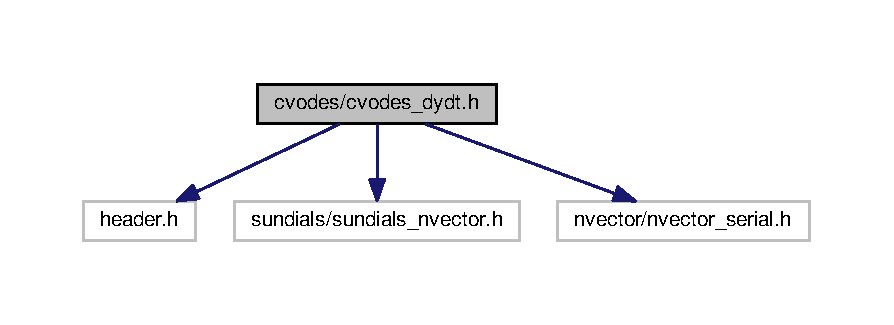
\includegraphics[width=350pt]{cvodes__dydt_8h__incl}
\end{center}
\end{figure}
This graph shows which files directly or indirectly include this file\+:\nopagebreak
\begin{figure}[H]
\begin{center}
\leavevmode
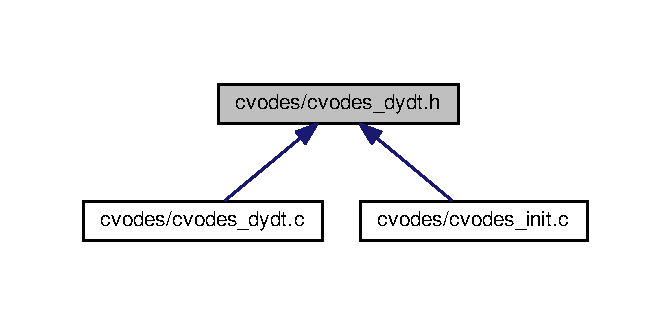
\includegraphics[width=195pt]{cvodes__dydt_8h__dep__incl}
\end{center}
\end{figure}
\subsection*{Functions}
\begin{DoxyCompactItemize}
\item 
int \hyperlink{cvodes__dydt_8h_ae27d76b55607dee9941b4d4e9962e065}{dydt\+\_\+cvodes} (double t, N\+\_\+\+Vector y, N\+\_\+\+Vector ydot, void $\ast$f)
\begin{DoxyCompactList}\small\item\em The C\+V\+O\+D\+Es R\+HS interface. \end{DoxyCompactList}\end{DoxyCompactItemize}


\subsection{Detailed Description}
Header file for C\+V\+O\+D\+Es interface to R\+HS of O\+D\+Es. 

This defines an interface to the right hand side of the O\+D\+Es to pass to C\+V\+O\+D\+Es 

\subsection{Function Documentation}
\index{cvodes\+\_\+dydt.\+h@{cvodes\+\_\+dydt.\+h}!dydt\+\_\+cvodes@{dydt\+\_\+cvodes}}
\index{dydt\+\_\+cvodes@{dydt\+\_\+cvodes}!cvodes\+\_\+dydt.\+h@{cvodes\+\_\+dydt.\+h}}
\subsubsection[{\texorpdfstring{dydt\+\_\+cvodes(double t, N\+\_\+\+Vector y, N\+\_\+\+Vector ydot, void $\ast$f)}{dydt_cvodes(double t, N_Vector y, N_Vector ydot, void *f)}}]{\setlength{\rightskip}{0pt plus 5cm}int dydt\+\_\+cvodes (
\begin{DoxyParamCaption}
\item[{double}]{t, }
\item[{N\+\_\+\+Vector}]{y, }
\item[{N\+\_\+\+Vector}]{ydot, }
\item[{void $\ast$}]{f}
\end{DoxyParamCaption}
)}\hypertarget{cvodes__dydt_8h_ae27d76b55607dee9941b4d4e9962e065}{}\label{cvodes__dydt_8h_ae27d76b55607dee9941b4d4e9962e065}


The C\+V\+O\+D\+Es R\+HS interface. 


\begin{DoxyParams}{Parameters}
{\em t} & The current time of the system \\
\hline
{\em y} & The current state vector (in C\+V\+O\+DE format) \\
\hline
{\em ydot} & The R\+HS vector to be populated (in C\+V\+O\+DE format) \\
\hline
{\em f} & User data set during C\+V\+O\+D\+Es setup (e.\+g. the system pressure) \\
\hline
\end{DoxyParams}
\begin{DoxyReturn}{Returns}
cvode\+\_\+return\+\_\+code The C\+V\+O\+DE output constant returned (see sec B.\+2 of C\+V\+O\+DE documentation), currently always returns C\+V\+\_\+\+S\+U\+C\+C\+E\+SS 
\end{DoxyReturn}

\hypertarget{cvodes__init_8c}{}\section{cvodes/cvodes\+\_\+init.c File Reference}
\label{cvodes__init_8c}\index{cvodes/cvodes\+\_\+init.\+c@{cvodes/cvodes\+\_\+init.\+c}}


Implementation of the necessary initialization for the C\+V\+O\+DE interface.  


{\ttfamily \#include \char`\"{}header.\+h\char`\"{}}\\*
{\ttfamily \#include \char`\"{}solver\+\_\+options.\+h\char`\"{}}\\*
{\ttfamily \#include \char`\"{}cvodes\+\_\+dydt.\+h\char`\"{}}\\*
{\ttfamily \#include \char`\"{}cvodes\+\_\+jac.\+h\char`\"{}}\\*
{\ttfamily \#include \char`\"{}sundials/sundials\+\_\+types.\+h\char`\"{}}\\*
{\ttfamily \#include \char`\"{}sundials/sundials\+\_\+math.\+h\char`\"{}}\\*
{\ttfamily \#include \char`\"{}sundials/sundials\+\_\+nvector.\+h\char`\"{}}\\*
{\ttfamily \#include \char`\"{}nvector/nvector\+\_\+serial.\+h\char`\"{}}\\*
{\ttfamily \#include \char`\"{}cvodes/cvodes.\+h\char`\"{}}\\*
{\ttfamily \#include \char`\"{}cvodes/cvodes\+\_\+lapack.\+h\char`\"{}}\\*
Include dependency graph for cvodes\+\_\+init.\+c\+:\nopagebreak
\begin{figure}[H]
\begin{center}
\leavevmode
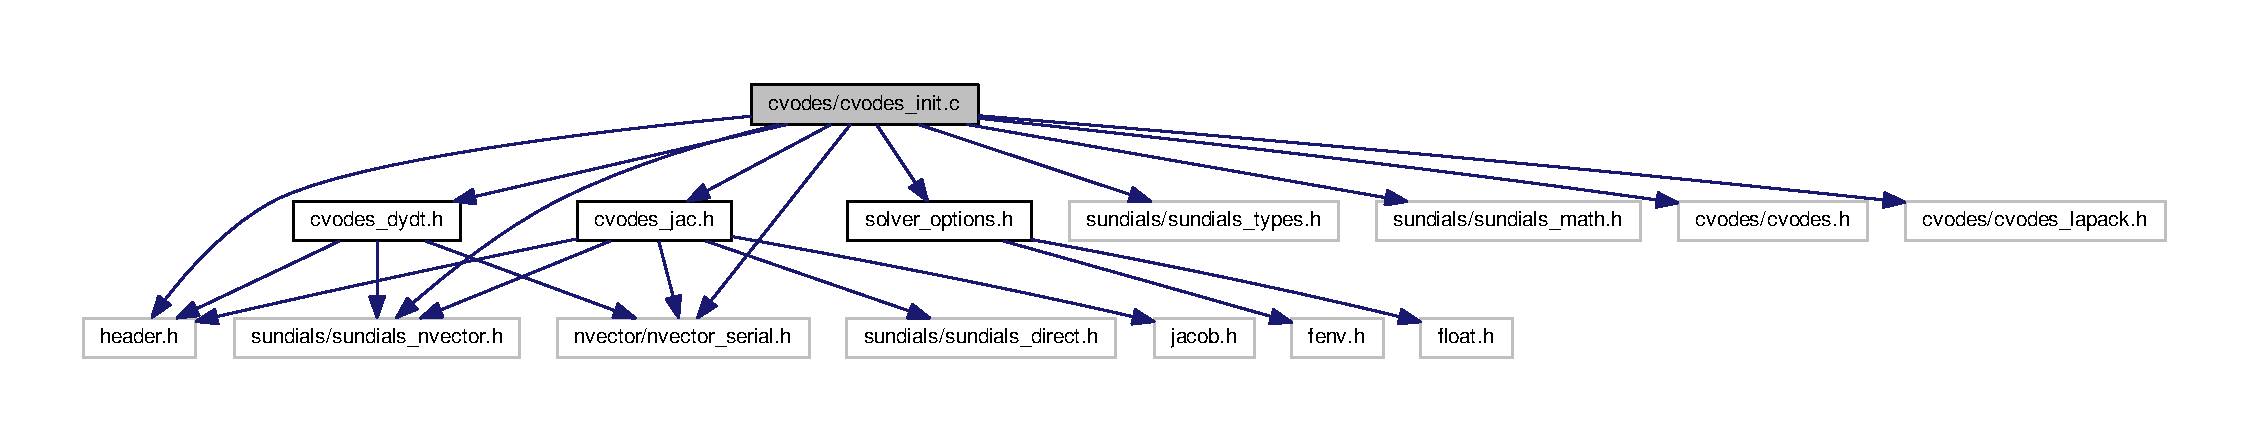
\includegraphics[width=350pt]{cvodes__init_8c__incl}
\end{center}
\end{figure}
\subsection*{Namespaces}
\begin{DoxyCompactItemize}
\item 
 \hyperlink{namespacecvode}{cvode}
\end{DoxyCompactItemize}
\subsection*{Functions}
\begin{DoxyCompactItemize}
\item 
int \hyperlink{namespacecvode_aa10a063b2a82d5b49c2bb338f16ddae4}{cvode\+::dydt\+\_\+cvodes} (double t, N\+\_\+\+Vector y, N\+\_\+\+Vector ydot, void $\ast$f)
\begin{DoxyCompactList}\small\item\em The C\+V\+O\+D\+Es R\+HS interface. \end{DoxyCompactList}\item 
int \hyperlink{namespacecvode_ab2efc395730d25bedc496a62e7896d24}{cvode\+::eval\+\_\+jacob\+\_\+cvodes} (long int N, double t, N\+\_\+\+Vector y, N\+\_\+\+Vector ydot, Dls\+Mat Jac, void $\ast$f, N\+\_\+\+Vector tmp1, N\+\_\+\+Vector tmp2, N\+\_\+\+Vector tmp3)
\begin{DoxyCompactList}\small\item\em The C\+V\+O\+D\+Es Jacobian interface for a direct dense Jacobian. \end{DoxyCompactList}\item 
void \hyperlink{namespacecvode_abe146525cea80d8032cd30b4441b5872}{cvode\+::initialize\+\_\+solver} (int num\+\_\+threads)
\begin{DoxyCompactList}\small\item\em Creates/\+Checks the C\+V\+O\+DE solvers for the specified number of threads. \end{DoxyCompactList}\item 
void \hyperlink{namespacecvode_ac9bc4957bff6721dae9d7e4cc470d184}{cvode\+::cleanup\+\_\+solver} (int num\+\_\+threads)
\begin{DoxyCompactList}\small\item\em Cleans up the created C\+V\+O\+DE solvers. \end{DoxyCompactList}\item 
const char $\ast$ \hyperlink{namespacecvode_a3a26024b8dc2ce6f8b2afcfb7c82c79f}{cvode\+::solver\+\_\+name} ()
\begin{DoxyCompactList}\small\item\em Returns the C\+V\+O\+DE solver name. \end{DoxyCompactList}\item 
void \hyperlink{namespacecvode_a9113d5fb0e19fa927d73b64c397ecd09}{cvode\+::init\+\_\+solver\+\_\+log} ()
\item 
void \hyperlink{namespacecvode_af7eb796b6829fecab506fb6dfec39be0}{cvode\+::solver\+\_\+log} ()
\end{DoxyCompactItemize}
\subsection*{Variables}
\begin{DoxyCompactItemize}
\item 
N\+\_\+\+Vector $\ast$ \hyperlink{namespacecvode_a84c47b6a9f2bedf2c5c80429079fc8e3}{cvode\+::y\+\_\+locals}
\item 
double $\ast$ \hyperlink{namespacecvode_adae183039534044ead74e1c1a786a36c}{cvode\+::y\+\_\+local\+\_\+vectors}
\item 
void $\ast$$\ast$ \hyperlink{namespacecvode_a9290e27651628dff03f82f42eafd3079}{cvode\+::integrators}
\end{DoxyCompactItemize}


\subsection{Detailed Description}
Implementation of the necessary initialization for the C\+V\+O\+DE interface. 

\begin{DoxyAuthor}{Author}
Nicholas Curtis 
\end{DoxyAuthor}
\begin{DoxyDate}{Date}
03/09/2015 
\end{DoxyDate}

\hypertarget{cvodes__jac_8c}{}\section{cvodes/cvodes\+\_\+jac.c File Reference}
\label{cvodes__jac_8c}\index{cvodes/cvodes\+\_\+jac.\+c@{cvodes/cvodes\+\_\+jac.\+c}}


A simple wrapper, allowing for use of the analytical jacobian w/ C\+V\+O\+D\+ES.  


{\ttfamily \#include \char`\"{}cvodes\+\_\+jac.\+h\char`\"{}}\\*
Include dependency graph for cvodes\+\_\+jac.\+c\+:\nopagebreak
\begin{figure}[H]
\begin{center}
\leavevmode
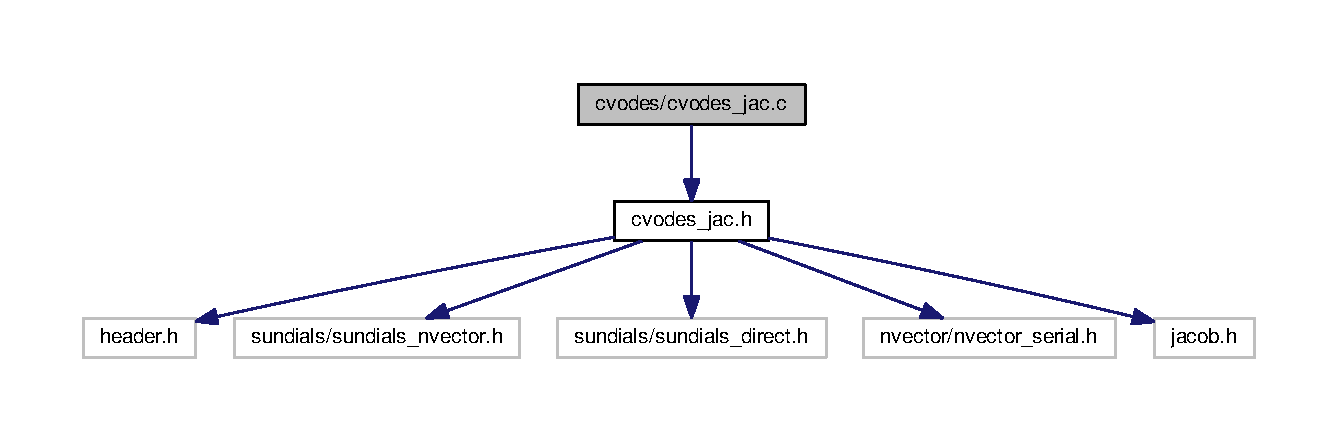
\includegraphics[width=350pt]{cvodes__jac_8c__incl}
\end{center}
\end{figure}
\subsection*{Functions}
\begin{DoxyCompactItemize}
\item 
int \hyperlink{cvodes__jac_8c_a25a1370ef7b8492e115d1ff20863d318}{eval\+\_\+jacob\+\_\+cvodes} (long int N, double t, N\+\_\+\+Vector y, N\+\_\+\+Vector ydot, Dls\+Mat jac, void $\ast$f, N\+\_\+\+Vector tmp1, N\+\_\+\+Vector tmp2, N\+\_\+\+Vector tmp3)
\begin{DoxyCompactList}\small\item\em The C\+V\+O\+D\+Es Jacobian interface for a direct dense Jacobian. \end{DoxyCompactList}\end{DoxyCompactItemize}


\subsection{Detailed Description}
A simple wrapper, allowing for use of the analytical jacobian w/ C\+V\+O\+D\+ES. 



\subsection{Function Documentation}
\index{cvodes\+\_\+jac.\+c@{cvodes\+\_\+jac.\+c}!eval\+\_\+jacob\+\_\+cvodes@{eval\+\_\+jacob\+\_\+cvodes}}
\index{eval\+\_\+jacob\+\_\+cvodes@{eval\+\_\+jacob\+\_\+cvodes}!cvodes\+\_\+jac.\+c@{cvodes\+\_\+jac.\+c}}
\subsubsection[{\texorpdfstring{eval\+\_\+jacob\+\_\+cvodes(long int N, double t, N\+\_\+\+Vector y, N\+\_\+\+Vector ydot, Dls\+Mat jac, void $\ast$f, N\+\_\+\+Vector tmp1, N\+\_\+\+Vector tmp2, N\+\_\+\+Vector tmp3)}{eval_jacob_cvodes(long int N, double t, N_Vector y, N_Vector ydot, DlsMat jac, void *f, N_Vector tmp1, N_Vector tmp2, N_Vector tmp3)}}]{\setlength{\rightskip}{0pt plus 5cm}int eval\+\_\+jacob\+\_\+cvodes (
\begin{DoxyParamCaption}
\item[{long int}]{N, }
\item[{double}]{t, }
\item[{N\+\_\+\+Vector}]{y, }
\item[{N\+\_\+\+Vector}]{ydot, }
\item[{Dls\+Mat}]{jac, }
\item[{void $\ast$}]{f, }
\item[{N\+\_\+\+Vector}]{tmp1, }
\item[{N\+\_\+\+Vector}]{tmp2, }
\item[{N\+\_\+\+Vector}]{tmp3}
\end{DoxyParamCaption}
)}\hypertarget{cvodes__jac_8c_a25a1370ef7b8492e115d1ff20863d318}{}\label{cvodes__jac_8c_a25a1370ef7b8492e115d1ff20863d318}


The C\+V\+O\+D\+Es Jacobian interface for a direct dense Jacobian. 

This function converts the N\+\_\+\+Vectors {\ttfamily y} and {\ttfamily y\+\_\+dot} to simple double pointers, the user data {\ttfamily f} to a double and outputs the Jacobian supplied by {\ttfamily eval\+\_\+jacob} to the C\+V\+O\+DE jacobian {\ttfamily jac} Currently, C\+V\+\_\+\+S\+U\+C\+C\+E\+SS is always returned. 
\hypertarget{cvodes__jac_8h}{}\section{cvodes/cvodes\+\_\+jac.h File Reference}
\label{cvodes__jac_8h}\index{cvodes/cvodes\+\_\+jac.\+h@{cvodes/cvodes\+\_\+jac.\+h}}


A simple wrapper, allowing for use of the analytical jacobian w/ C\+V\+O\+D\+ES.  


{\ttfamily \#include \char`\"{}header.\+h\char`\"{}}\\*
{\ttfamily \#include \char`\"{}sundials/sundials\+\_\+nvector.\+h\char`\"{}}\\*
{\ttfamily \#include \char`\"{}sundials/sundials\+\_\+direct.\+h\char`\"{}}\\*
{\ttfamily \#include \char`\"{}nvector/nvector\+\_\+serial.\+h\char`\"{}}\\*
{\ttfamily \#include \char`\"{}jacob.\+h\char`\"{}}\\*
Include dependency graph for cvodes\+\_\+jac.\+h\+:\nopagebreak
\begin{figure}[H]
\begin{center}
\leavevmode
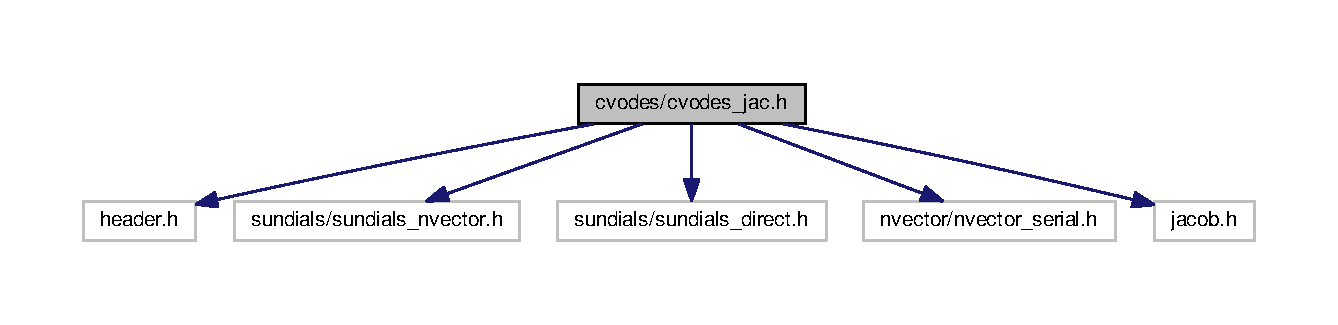
\includegraphics[width=350pt]{cvodes__jac_8h__incl}
\end{center}
\end{figure}
This graph shows which files directly or indirectly include this file\+:\nopagebreak
\begin{figure}[H]
\begin{center}
\leavevmode
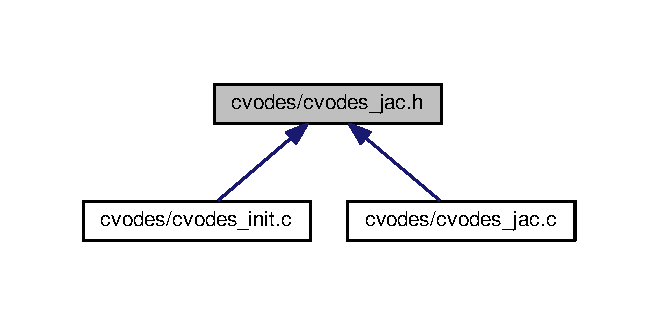
\includegraphics[width=316pt]{cvodes__jac_8h__dep__incl}
\end{center}
\end{figure}
\subsection*{Macros}
\begin{DoxyCompactItemize}
\item 
\#define \hyperlink{cvodes__init_8c_afc974a5ba6f507ebbdeb4dd3f8c5abdc}{J\+A\+C\+\_\+\+H\+E\+A\+D\+\_\+\+C\+V\+O\+D\+ES}
\end{DoxyCompactItemize}
\subsection*{Functions}
\begin{DoxyCompactItemize}
\item 
int \hyperlink{cvodes__jac_8h_ace0ee8931b5755b80309735167af0b86}{eval\+\_\+jacob\+\_\+cvodes} (long int N, double t, N\+\_\+\+Vector y, N\+\_\+\+Vector ydot, Dls\+Mat Jac, void $\ast$f, N\+\_\+\+Vector tmp1, N\+\_\+\+Vector tmp2, N\+\_\+\+Vector tmp3)
\begin{DoxyCompactList}\small\item\em The C\+V\+O\+D\+Es Jacobian interface for a direct dense Jacobian. \end{DoxyCompactList}\end{DoxyCompactItemize}


\subsection{Detailed Description}
A simple wrapper, allowing for use of the analytical jacobian w/ C\+V\+O\+D\+ES. 



\subsection{Macro Definition Documentation}
\index{cvodes\+\_\+jac.\+h@{cvodes\+\_\+jac.\+h}!J\+A\+C\+\_\+\+H\+E\+A\+D\+\_\+\+C\+V\+O\+D\+ES@{J\+A\+C\+\_\+\+H\+E\+A\+D\+\_\+\+C\+V\+O\+D\+ES}}
\index{J\+A\+C\+\_\+\+H\+E\+A\+D\+\_\+\+C\+V\+O\+D\+ES@{J\+A\+C\+\_\+\+H\+E\+A\+D\+\_\+\+C\+V\+O\+D\+ES}!cvodes\+\_\+jac.\+h@{cvodes\+\_\+jac.\+h}}
\subsubsection[{\texorpdfstring{J\+A\+C\+\_\+\+H\+E\+A\+D\+\_\+\+C\+V\+O\+D\+ES}{JAC_HEAD_CVODES}}]{\setlength{\rightskip}{0pt plus 5cm}\#define J\+A\+C\+\_\+\+H\+E\+A\+D\+\_\+\+C\+V\+O\+D\+ES}\hypertarget{cvodes__init_8c_afc974a5ba6f507ebbdeb4dd3f8c5abdc}{}\label{cvodes__init_8c_afc974a5ba6f507ebbdeb4dd3f8c5abdc}


\subsection{Function Documentation}
\index{cvodes\+\_\+jac.\+h@{cvodes\+\_\+jac.\+h}!eval\+\_\+jacob\+\_\+cvodes@{eval\+\_\+jacob\+\_\+cvodes}}
\index{eval\+\_\+jacob\+\_\+cvodes@{eval\+\_\+jacob\+\_\+cvodes}!cvodes\+\_\+jac.\+h@{cvodes\+\_\+jac.\+h}}
\subsubsection[{\texorpdfstring{eval\+\_\+jacob\+\_\+cvodes(long int N, double t, N\+\_\+\+Vector y, N\+\_\+\+Vector ydot, Dls\+Mat Jac, void $\ast$f, N\+\_\+\+Vector tmp1, N\+\_\+\+Vector tmp2, N\+\_\+\+Vector tmp3)}{eval_jacob_cvodes(long int N, double t, N_Vector y, N_Vector ydot, DlsMat Jac, void *f, N_Vector tmp1, N_Vector tmp2, N_Vector tmp3)}}]{\setlength{\rightskip}{0pt plus 5cm}int eval\+\_\+jacob\+\_\+cvodes (
\begin{DoxyParamCaption}
\item[{long int}]{N, }
\item[{double}]{t, }
\item[{N\+\_\+\+Vector}]{y, }
\item[{N\+\_\+\+Vector}]{ydot, }
\item[{Dls\+Mat}]{jac, }
\item[{void $\ast$}]{f, }
\item[{N\+\_\+\+Vector}]{tmp1, }
\item[{N\+\_\+\+Vector}]{tmp2, }
\item[{N\+\_\+\+Vector}]{tmp3}
\end{DoxyParamCaption}
)}\hypertarget{cvodes__jac_8h_ace0ee8931b5755b80309735167af0b86}{}\label{cvodes__jac_8h_ace0ee8931b5755b80309735167af0b86}


The C\+V\+O\+D\+Es Jacobian interface for a direct dense Jacobian. 


\begin{DoxyParams}{Parameters}
{\em N} & the problem size \\
\hline
{\em t} & The current time of the system \\
\hline
{\em y} & The current state vector (in C\+V\+O\+DE format) \\
\hline
{\em ydot} & The R\+HS vector to be populated (in C\+V\+O\+DE format) \\
\hline
{\em jac} & The Jacobian matrix (in C\+V\+O\+DE format) to output to \\
\hline
{\em f} & User data set during C\+V\+O\+D\+Es setup (e.\+g. the system pressure) \\
\hline
{\em tmp1} & Temporary storage used by C\+V\+O\+D\+Es \\
\hline
{\em tmp2} & Temporary storage used by C\+V\+O\+D\+Es \\
\hline
{\em tmp3} & Temporary storage used by C\+V\+O\+D\+Es \\
\hline
\end{DoxyParams}
\begin{DoxyReturn}{Returns}
cvode\+\_\+return\+\_\+code The C\+V\+O\+DE output constant returned (see sec B.\+2 of C\+V\+O\+DE documentation), currently always returns C\+V\+\_\+\+S\+U\+C\+C\+E\+SS
\end{DoxyReturn}
This function converts the N\+\_\+\+Vectors {\ttfamily y} and {\ttfamily y\+\_\+dot} to simple double pointers, the user data {\ttfamily f} to a double and outputs the Jacobian supplied by {\ttfamily eval\+\_\+jacob} to the C\+V\+O\+DE jacobian {\ttfamily jac} Currently, C\+V\+\_\+\+S\+U\+C\+C\+E\+SS is always returned. 
\hypertarget{cf_8c}{}\section{exponential\+\_\+integrators/cf.c File Reference}
\label{cf_8c}\index{exponential\+\_\+integrators/cf.\+c@{exponential\+\_\+integrators/cf.\+c}}
{\ttfamily \#include $<$stdlib.\+h$>$}\\*
{\ttfamily \#include $<$math.\+h$>$}\\*
{\ttfamily \#include $<$string.\+h$>$}\\*
{\ttfamily \#include \char`\"{}solver\+\_\+options.\+h\char`\"{}}\\*
{\ttfamily \#include \char`\"{}linear-\/algebra.\+h\char`\"{}}\\*
{\ttfamily \#include $<$complex.\+h$>$}\\*
{\ttfamily \#include $<$fftw3.\+h$>$}\\*
Include dependency graph for cf.\+c\+:\nopagebreak
\begin{figure}[H]
\begin{center}
\leavevmode
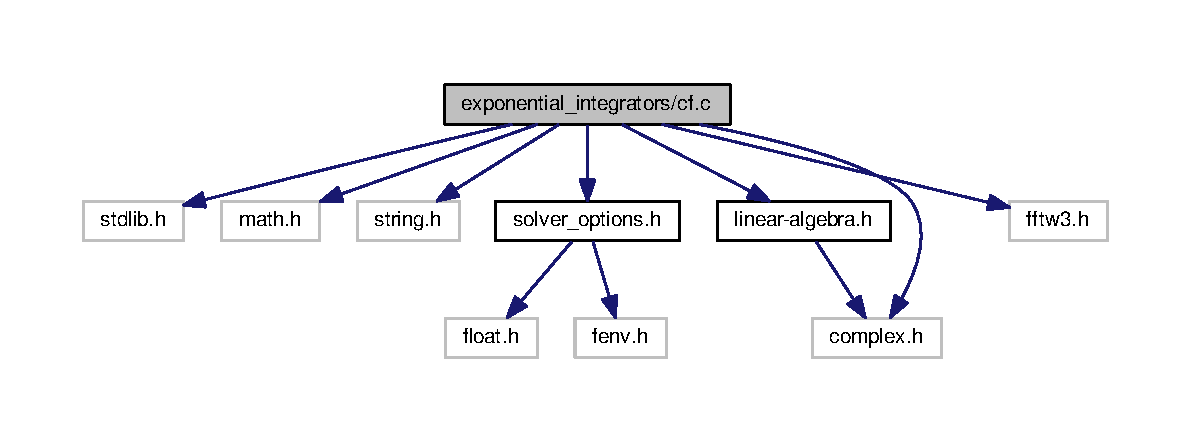
\includegraphics[width=350pt]{cf_8c__incl}
\end{center}
\end{figure}
\subsection*{Macros}
\begin{DoxyCompactItemize}
\item 
\#define \hyperlink{cf_8c_ae71449b1cc6e6250b91f539153a7a0d3}{M\+\_\+\+PI}~4 $\ast$ atan(1)
\end{DoxyCompactItemize}
\subsection*{Functions}
\begin{DoxyCompactItemize}
\item 
void \hyperlink{cf_8c_a8fe7eda5752653bf298684fbe6a18045}{cf} (int n, double $\ast$poles\+\_\+r, double $\ast$poles\+\_\+i, double $\ast$res\+\_\+r, double $\ast$res\+\_\+i)
\begin{DoxyCompactList}\small\item\em Function that calculates the poles and residuals of best rational (partial fraction) approximant to the matrix exponential. \end{DoxyCompactList}\end{DoxyCompactItemize}


\subsection{Detailed Description}
File containing functions for best rational approximation to matrix exponential.

\begin{DoxyAuthor}{Author}
Kyle E. Niemeyer 
\end{DoxyAuthor}
\begin{DoxyDate}{Date}
07/19/2012
\end{DoxyDate}
Contains main and linear algebra functions. 

\subsection{Macro Definition Documentation}
\index{cf.\+c@{cf.\+c}!M\+\_\+\+PI@{M\+\_\+\+PI}}
\index{M\+\_\+\+PI@{M\+\_\+\+PI}!cf.\+c@{cf.\+c}}
\subsubsection[{\texorpdfstring{M\+\_\+\+PI}{M_PI}}]{\setlength{\rightskip}{0pt plus 5cm}\#define M\+\_\+\+PI~4 $\ast$ atan(1)}\hypertarget{cf_8c_ae71449b1cc6e6250b91f539153a7a0d3}{}\label{cf_8c_ae71449b1cc6e6250b91f539153a7a0d3}
Defined for pi 

\subsection{Function Documentation}
\index{cf.\+c@{cf.\+c}!cf@{cf}}
\index{cf@{cf}!cf.\+c@{cf.\+c}}
\subsubsection[{\texorpdfstring{cf(int n, double $\ast$poles\+\_\+r, double $\ast$poles\+\_\+i, double $\ast$res\+\_\+r, double $\ast$res\+\_\+i)}{cf(int n, double *poles_r, double *poles_i, double *res_r, double *res_i)}}]{\setlength{\rightskip}{0pt plus 5cm}void cf (
\begin{DoxyParamCaption}
\item[{int}]{n, }
\item[{double $\ast$}]{poles\+\_\+r, }
\item[{double $\ast$}]{poles\+\_\+i, }
\item[{double $\ast$}]{res\+\_\+r, }
\item[{double $\ast$}]{res\+\_\+i}
\end{DoxyParamCaption}
)}\hypertarget{cf_8c_a8fe7eda5752653bf298684fbe6a18045}{}\label{cf_8c_a8fe7eda5752653bf298684fbe6a18045}


Function that calculates the poles and residuals of best rational (partial fraction) approximant to the matrix exponential. 

Complex math Fast Fourier tranform functions\+Uses the Carathéodory-\/\+Fejér method; based on the M\+A\+T\+L\+AB code in L.\+N. Trefethen, J.\+A.\+C. Weideman, T. Schmelzer, \char`\"{}\+Talbot quadratures
and rational approximations,\char`\"{} B\+IT Numer. Math. 46 (2006) 653–670.


\begin{DoxyParams}[1]{Parameters}
\mbox{\tt in}  & {\em n} & size of approximation (n, n) \\
\hline
\mbox{\tt out}  & {\em poles\+\_\+r} & array with real parts of poles, size n \\
\hline
\mbox{\tt out}  & {\em poles\+\_\+i} & array with imaginary parts of poles, size n \\
\hline
\mbox{\tt out}  & {\em res\+\_\+r} & array with real parts of residuals, size n \\
\hline
\mbox{\tt out}  & {\em res\+\_\+i} & array with imaginary parts of residuals, size n \\
\hline
\end{DoxyParams}

\hypertarget{solver__options_8cuh}{}\section{generic/solver\+\_\+options.cuh File Reference}
\label{solver__options_8cuh}\index{generic/solver\+\_\+options.\+cuh@{generic/solver\+\_\+options.\+cuh}}


A file generated by Scons that specifies various options to the solvers.  


{\ttfamily \#include $<$float.\+h$>$}\\*
{\ttfamily \#include $<$fenv.\+h$>$}\\*
Include dependency graph for solver\+\_\+options.\+cuh\+:\nopagebreak
\begin{figure}[H]
\begin{center}
\leavevmode
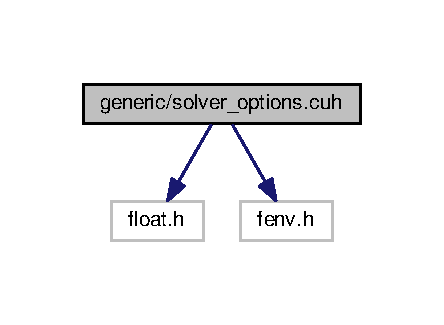
\includegraphics[width=213pt]{solver__options_8cuh__incl}
\end{center}
\end{figure}
This graph shows which files directly or indirectly include this file\+:\nopagebreak
\begin{figure}[H]
\begin{center}
\leavevmode
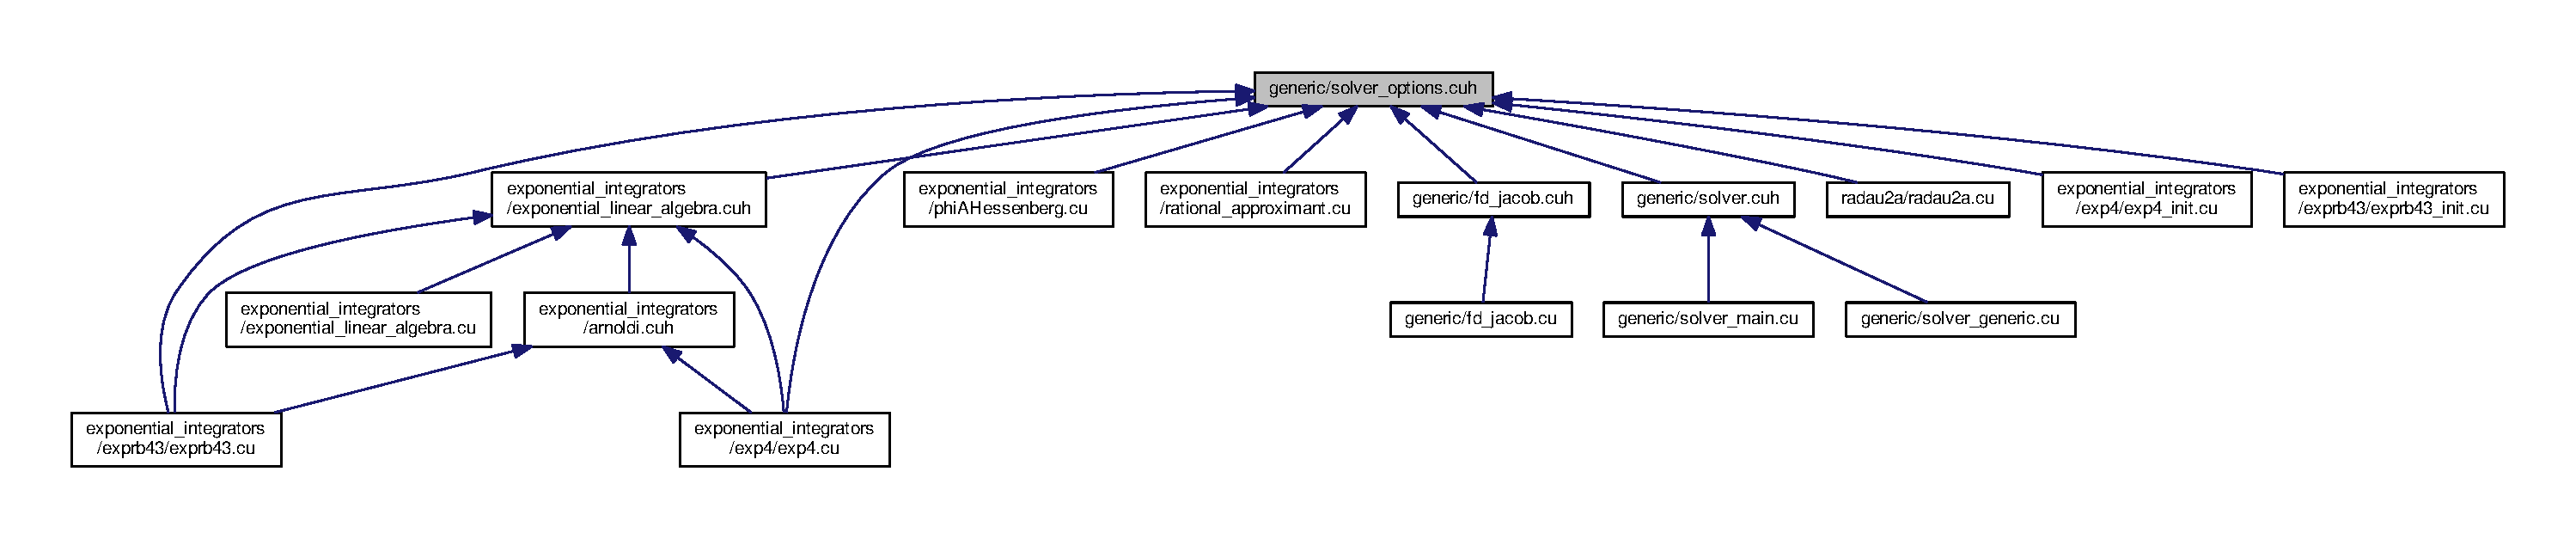
\includegraphics[width=213pt]{solver__options_8cuh__dep__incl}
\end{center}
\end{figure}
\subsection*{Macros}
\begin{DoxyCompactItemize}
\item 
\#define {\bfseries S\+O\+L\+V\+\_\+\+O\+P\+T\+\_\+\+H\+E\+AD}\hypertarget{solver__options_8cuh_a0cdb20d794f10fb22eebe8854ae6aa45}{}\label{solver__options_8cuh_a0cdb20d794f10fb22eebe8854ae6aa45}

\item 
\#define \hyperlink{solver__options_8cuh_a29a15cd00b37b1f4a5b4ec9f07c742f4}{A\+T\+OL}~(1e-\/10)
\item 
\#define \hyperlink{solver__options_8cuh_af50ac611d9fae906f9419504fd2caa5d}{R\+T\+OL}~(1e-\/06)
\item 
\#define \hyperlink{solver__options_8cuh_aaeb7127cf3bf0b49cec6554fbc101866}{t\+\_\+step}~(1e-\/06)
\item 
\#define \hyperlink{solver__options_8cuh_a25526ead9bdb589c90e7a8d3b4d1a746}{end\+\_\+time}~(1e-\/06)
\item 
\#define \hyperlink{solver__options_8cuh_a6ebf6899d6c1c8b7b9d09be872c05aae}{E\+PS}~D\+B\+L\+\_\+\+E\+P\+S\+I\+L\+ON
\item 
\#define \hyperlink{solver__options_8cuh_a09c78d2f8feb311dd9fc969a0bf84979}{S\+M\+A\+LL}~D\+B\+L\+\_\+\+M\+IN
\item 
\#define \hyperlink{solver__options_8cuh_a69f5533c684b73d07a7e20146a285cb1}{N\+\_\+\+RA}~(10)
\item 
\#define \hyperlink{solver__options_8cuh_a8dd330cbca99d70609ccc451d9099383}{C\+V\+\_\+\+M\+A\+X\+\_\+\+S\+T\+E\+PS}~(-\/1)
\item 
\#define \hyperlink{solver__options_8cuh_af45d9c410d5d7c99d2692080832d506e}{C\+V\+\_\+\+M\+A\+X\+\_\+\+H\+N\+IL}~(1)
\item 
\#define \hyperlink{solver__options_8cuh_ac42e0287ba619ab25b7d767a81f48082}{C\+V\+\_\+\+M\+A\+X\+\_\+\+E\+R\+R\+T\+E\+S\+T\+\_\+\+F\+A\+I\+LS}~(5)
\item 
\#define \hyperlink{solver__options_8cuh_aa98acf0dc83a3dce3ba168d75a74cb1b}{S\+A\+M\+E\+\_\+\+IC}
\item 
\#define \hyperlink{solver__options_8cuh_ad72dbcf6d0153db1b8d8a58001feed83}{D\+E\+B\+UG}
\item 
\#define \hyperlink{solver__options_8cuh_a0b43a0be2f674fea3218e7fb5221db1f}{S\+H\+U\+F\+F\+LE}
\item 
\#define \hyperlink{solver__options_8cuh_a8b43bafee90b30676faae508c21cb8d7}{P\+R\+I\+NT}
\item 
\#define \hyperlink{solver__options_8cuh_af5cccef89d39980a452b7f3a7c59fb53}{I\+GN}
\item 
\#define \hyperlink{solver__options_8cuh_ac786f5f1963363a48eed565f7cbc6931}{L\+O\+G\+\_\+\+O\+U\+T\+P\+UT}
\item 
\#define \hyperlink{solver__options_8cuh_a2adffa059bbd6f183ff7f63db602ac42}{L\+O\+G\+\_\+\+K\+R\+Y\+L\+O\+V\+\_\+\+A\+N\+D\+\_\+\+S\+T\+E\+P\+S\+I\+Z\+ES}
\item 
\#define \hyperlink{solver__options_8cuh_a09cc461392fae3949d88392adf655db5}{L\+O\+G\+\_\+\+E\+N\+D\+\_\+\+O\+N\+LY}
\item 
\#define \hyperlink{solver__options_8cuh_a9e28db46fb24c2d46dbfe205c6a11236}{F\+I\+N\+I\+T\+E\+\_\+\+D\+I\+F\+F\+E\+R\+E\+N\+CE}
\item 
\#define \hyperlink{solver__options_8cuh_afd8c973bc66908100d15f47ae514ed41}{D\+I\+V\+E\+R\+G\+E\+N\+C\+E\+\_\+\+T\+E\+ST}~(2048 $\ast$ 32)
\item 
\#define \hyperlink{solver__options_8cuh_a66c8290aad471b0be7768f635f03c349}{C\+O\+N\+S\+T\+\_\+\+T\+I\+M\+E\+\_\+\+S\+T\+EP}
\end{DoxyCompactItemize}


\subsection{Detailed Description}
A file generated by Scons that specifies various options to the solvers. 

This file, autogenerated by S\+Cons contains a number of definitions that can be enabled via command line options. These control the integrator behaviour and alternately enable special behaviour such as logging, divergence measuring, etc.

Note that it is not typical for all these options to be turned on at the same time, but it is done here for documentation purposes. 

\subsection{Macro Definition Documentation}
\index{solver\+\_\+options.\+cuh@{solver\+\_\+options.\+cuh}!A\+T\+OL@{A\+T\+OL}}
\index{A\+T\+OL@{A\+T\+OL}!solver\+\_\+options.\+cuh@{solver\+\_\+options.\+cuh}}
\subsubsection[{\texorpdfstring{A\+T\+OL}{ATOL}}]{\setlength{\rightskip}{0pt plus 5cm}\#define A\+T\+OL~(1e-\/10)}\hypertarget{solver__options_8cuh_a29a15cd00b37b1f4a5b4ec9f07c742f4}{}\label{solver__options_8cuh_a29a15cd00b37b1f4a5b4ec9f07c742f4}
Absolute solver tolerance \index{solver\+\_\+options.\+cuh@{solver\+\_\+options.\+cuh}!C\+O\+N\+S\+T\+\_\+\+T\+I\+M\+E\+\_\+\+S\+T\+EP@{C\+O\+N\+S\+T\+\_\+\+T\+I\+M\+E\+\_\+\+S\+T\+EP}}
\index{C\+O\+N\+S\+T\+\_\+\+T\+I\+M\+E\+\_\+\+S\+T\+EP@{C\+O\+N\+S\+T\+\_\+\+T\+I\+M\+E\+\_\+\+S\+T\+EP}!solver\+\_\+options.\+cuh@{solver\+\_\+options.\+cuh}}
\subsubsection[{\texorpdfstring{C\+O\+N\+S\+T\+\_\+\+T\+I\+M\+E\+\_\+\+S\+T\+EP}{CONST_TIME_STEP}}]{\setlength{\rightskip}{0pt plus 5cm}\#define C\+O\+N\+S\+T\+\_\+\+T\+I\+M\+E\+\_\+\+S\+T\+EP}\hypertarget{solver__options_8cuh_a66c8290aad471b0be7768f635f03c349}{}\label{solver__options_8cuh_a66c8290aad471b0be7768f635f03c349}
Define to turn off adaptive time stepping \index{solver\+\_\+options.\+cuh@{solver\+\_\+options.\+cuh}!C\+V\+\_\+\+M\+A\+X\+\_\+\+E\+R\+R\+T\+E\+S\+T\+\_\+\+F\+A\+I\+LS@{C\+V\+\_\+\+M\+A\+X\+\_\+\+E\+R\+R\+T\+E\+S\+T\+\_\+\+F\+A\+I\+LS}}
\index{C\+V\+\_\+\+M\+A\+X\+\_\+\+E\+R\+R\+T\+E\+S\+T\+\_\+\+F\+A\+I\+LS@{C\+V\+\_\+\+M\+A\+X\+\_\+\+E\+R\+R\+T\+E\+S\+T\+\_\+\+F\+A\+I\+LS}!solver\+\_\+options.\+cuh@{solver\+\_\+options.\+cuh}}
\subsubsection[{\texorpdfstring{C\+V\+\_\+\+M\+A\+X\+\_\+\+E\+R\+R\+T\+E\+S\+T\+\_\+\+F\+A\+I\+LS}{CV_MAX_ERRTEST_FAILS}}]{\setlength{\rightskip}{0pt plus 5cm}\#define C\+V\+\_\+\+M\+A\+X\+\_\+\+E\+R\+R\+T\+E\+S\+T\+\_\+\+F\+A\+I\+LS~(5)}\hypertarget{solver__options_8cuh_ac42e0287ba619ab25b7d767a81f48082}{}\label{solver__options_8cuh_ac42e0287ba619ab25b7d767a81f48082}
Maximum number of C\+V\+O\+DE error test fails before an error is thrown \index{solver\+\_\+options.\+cuh@{solver\+\_\+options.\+cuh}!C\+V\+\_\+\+M\+A\+X\+\_\+\+H\+N\+IL@{C\+V\+\_\+\+M\+A\+X\+\_\+\+H\+N\+IL}}
\index{C\+V\+\_\+\+M\+A\+X\+\_\+\+H\+N\+IL@{C\+V\+\_\+\+M\+A\+X\+\_\+\+H\+N\+IL}!solver\+\_\+options.\+cuh@{solver\+\_\+options.\+cuh}}
\subsubsection[{\texorpdfstring{C\+V\+\_\+\+M\+A\+X\+\_\+\+H\+N\+IL}{CV_MAX_HNIL}}]{\setlength{\rightskip}{0pt plus 5cm}\#define C\+V\+\_\+\+M\+A\+X\+\_\+\+H\+N\+IL~(1)}\hypertarget{solver__options_8cuh_af45d9c410d5d7c99d2692080832d506e}{}\label{solver__options_8cuh_af45d9c410d5d7c99d2692080832d506e}
Number of t + h == t warnings emitted by C\+V\+O\+DE (used to cleanup output) \index{solver\+\_\+options.\+cuh@{solver\+\_\+options.\+cuh}!C\+V\+\_\+\+M\+A\+X\+\_\+\+S\+T\+E\+PS@{C\+V\+\_\+\+M\+A\+X\+\_\+\+S\+T\+E\+PS}}
\index{C\+V\+\_\+\+M\+A\+X\+\_\+\+S\+T\+E\+PS@{C\+V\+\_\+\+M\+A\+X\+\_\+\+S\+T\+E\+PS}!solver\+\_\+options.\+cuh@{solver\+\_\+options.\+cuh}}
\subsubsection[{\texorpdfstring{C\+V\+\_\+\+M\+A\+X\+\_\+\+S\+T\+E\+PS}{CV_MAX_STEPS}}]{\setlength{\rightskip}{0pt plus 5cm}\#define C\+V\+\_\+\+M\+A\+X\+\_\+\+S\+T\+E\+PS~(-\/1)}\hypertarget{solver__options_8cuh_a8dd330cbca99d70609ccc451d9099383}{}\label{solver__options_8cuh_a8dd330cbca99d70609ccc451d9099383}
Maximum steps the solver will take in one timestep set to -\/1 (disabled) by default \index{solver\+\_\+options.\+cuh@{solver\+\_\+options.\+cuh}!D\+E\+B\+UG@{D\+E\+B\+UG}}
\index{D\+E\+B\+UG@{D\+E\+B\+UG}!solver\+\_\+options.\+cuh@{solver\+\_\+options.\+cuh}}
\subsubsection[{\texorpdfstring{D\+E\+B\+UG}{DEBUG}}]{\setlength{\rightskip}{0pt plus 5cm}\#define D\+E\+B\+UG}\hypertarget{solver__options_8cuh_ad72dbcf6d0153db1b8d8a58001feed83}{}\label{solver__options_8cuh_ad72dbcf6d0153db1b8d8a58001feed83}
Turn on debugging symbols, and use O0 optimization \index{solver\+\_\+options.\+cuh@{solver\+\_\+options.\+cuh}!D\+I\+V\+E\+R\+G\+E\+N\+C\+E\+\_\+\+T\+E\+ST@{D\+I\+V\+E\+R\+G\+E\+N\+C\+E\+\_\+\+T\+E\+ST}}
\index{D\+I\+V\+E\+R\+G\+E\+N\+C\+E\+\_\+\+T\+E\+ST@{D\+I\+V\+E\+R\+G\+E\+N\+C\+E\+\_\+\+T\+E\+ST}!solver\+\_\+options.\+cuh@{solver\+\_\+options.\+cuh}}
\subsubsection[{\texorpdfstring{D\+I\+V\+E\+R\+G\+E\+N\+C\+E\+\_\+\+T\+E\+ST}{DIVERGENCE_TEST}}]{\setlength{\rightskip}{0pt plus 5cm}\#define D\+I\+V\+E\+R\+G\+E\+N\+C\+E\+\_\+\+T\+E\+ST~(2048 $\ast$ 32)}\hypertarget{solver__options_8cuh_afd8c973bc66908100d15f47ae514ed41}{}\label{solver__options_8cuh_afd8c973bc66908100d15f47ae514ed41}
Measure the thread divergence for this many initial conditions \index{solver\+\_\+options.\+cuh@{solver\+\_\+options.\+cuh}!end\+\_\+time@{end\+\_\+time}}
\index{end\+\_\+time@{end\+\_\+time}!solver\+\_\+options.\+cuh@{solver\+\_\+options.\+cuh}}
\subsubsection[{\texorpdfstring{end\+\_\+time}{end_time}}]{\setlength{\rightskip}{0pt plus 5cm}\#define end\+\_\+time~(1e-\/06)}\hypertarget{solver__options_8cuh_a25526ead9bdb589c90e7a8d3b4d1a746}{}\label{solver__options_8cuh_a25526ead9bdb589c90e7a8d3b4d1a746}
Global integration timestep \index{solver\+\_\+options.\+cuh@{solver\+\_\+options.\+cuh}!E\+PS@{E\+PS}}
\index{E\+PS@{E\+PS}!solver\+\_\+options.\+cuh@{solver\+\_\+options.\+cuh}}
\subsubsection[{\texorpdfstring{E\+PS}{EPS}}]{\setlength{\rightskip}{0pt plus 5cm}\#define E\+PS~D\+B\+L\+\_\+\+E\+P\+S\+I\+L\+ON}\hypertarget{solver__options_8cuh_a6ebf6899d6c1c8b7b9d09be872c05aae}{}\label{solver__options_8cuh_a6ebf6899d6c1c8b7b9d09be872c05aae}
Machine precision constant. \index{solver\+\_\+options.\+cuh@{solver\+\_\+options.\+cuh}!F\+I\+N\+I\+T\+E\+\_\+\+D\+I\+F\+F\+E\+R\+E\+N\+CE@{F\+I\+N\+I\+T\+E\+\_\+\+D\+I\+F\+F\+E\+R\+E\+N\+CE}}
\index{F\+I\+N\+I\+T\+E\+\_\+\+D\+I\+F\+F\+E\+R\+E\+N\+CE@{F\+I\+N\+I\+T\+E\+\_\+\+D\+I\+F\+F\+E\+R\+E\+N\+CE}!solver\+\_\+options.\+cuh@{solver\+\_\+options.\+cuh}}
\subsubsection[{\texorpdfstring{F\+I\+N\+I\+T\+E\+\_\+\+D\+I\+F\+F\+E\+R\+E\+N\+CE}{FINITE_DIFFERENCE}}]{\setlength{\rightskip}{0pt plus 5cm}\#define F\+I\+N\+I\+T\+E\+\_\+\+D\+I\+F\+F\+E\+R\+E\+N\+CE}\hypertarget{solver__options_8cuh_a9e28db46fb24c2d46dbfe205c6a11236}{}\label{solver__options_8cuh_a9e28db46fb24c2d46dbfe205c6a11236}
Use a Finite Difference Jaobian \index{solver\+\_\+options.\+cuh@{solver\+\_\+options.\+cuh}!I\+GN@{I\+GN}}
\index{I\+GN@{I\+GN}!solver\+\_\+options.\+cuh@{solver\+\_\+options.\+cuh}}
\subsubsection[{\texorpdfstring{I\+GN}{IGN}}]{\setlength{\rightskip}{0pt plus 5cm}\#define I\+GN}\hypertarget{solver__options_8cuh_af5cccef89d39980a452b7f3a7c59fb53}{}\label{solver__options_8cuh_af5cccef89d39980a452b7f3a7c59fb53}
Output ignition time (determined by simple T0 + 400 criteria) \index{solver\+\_\+options.\+cuh@{solver\+\_\+options.\+cuh}!L\+O\+G\+\_\+\+E\+N\+D\+\_\+\+O\+N\+LY@{L\+O\+G\+\_\+\+E\+N\+D\+\_\+\+O\+N\+LY}}
\index{L\+O\+G\+\_\+\+E\+N\+D\+\_\+\+O\+N\+LY@{L\+O\+G\+\_\+\+E\+N\+D\+\_\+\+O\+N\+LY}!solver\+\_\+options.\+cuh@{solver\+\_\+options.\+cuh}}
\subsubsection[{\texorpdfstring{L\+O\+G\+\_\+\+E\+N\+D\+\_\+\+O\+N\+LY}{LOG_END_ONLY}}]{\setlength{\rightskip}{0pt plus 5cm}\#define L\+O\+G\+\_\+\+E\+N\+D\+\_\+\+O\+N\+LY}\hypertarget{solver__options_8cuh_a09cc461392fae3949d88392adf655db5}{}\label{solver__options_8cuh_a09cc461392fae3949d88392adf655db5}
Log output to binary file only on final timestep \index{solver\+\_\+options.\+cuh@{solver\+\_\+options.\+cuh}!L\+O\+G\+\_\+\+K\+R\+Y\+L\+O\+V\+\_\+\+A\+N\+D\+\_\+\+S\+T\+E\+P\+S\+I\+Z\+ES@{L\+O\+G\+\_\+\+K\+R\+Y\+L\+O\+V\+\_\+\+A\+N\+D\+\_\+\+S\+T\+E\+P\+S\+I\+Z\+ES}}
\index{L\+O\+G\+\_\+\+K\+R\+Y\+L\+O\+V\+\_\+\+A\+N\+D\+\_\+\+S\+T\+E\+P\+S\+I\+Z\+ES@{L\+O\+G\+\_\+\+K\+R\+Y\+L\+O\+V\+\_\+\+A\+N\+D\+\_\+\+S\+T\+E\+P\+S\+I\+Z\+ES}!solver\+\_\+options.\+cuh@{solver\+\_\+options.\+cuh}}
\subsubsection[{\texorpdfstring{L\+O\+G\+\_\+\+K\+R\+Y\+L\+O\+V\+\_\+\+A\+N\+D\+\_\+\+S\+T\+E\+P\+S\+I\+Z\+ES}{LOG_KRYLOV_AND_STEPSIZES}}]{\setlength{\rightskip}{0pt plus 5cm}\#define L\+O\+G\+\_\+\+K\+R\+Y\+L\+O\+V\+\_\+\+A\+N\+D\+\_\+\+S\+T\+E\+P\+S\+I\+Z\+ES}\hypertarget{solver__options_8cuh_a2adffa059bbd6f183ff7f63db602ac42}{}\label{solver__options_8cuh_a2adffa059bbd6f183ff7f63db602ac42}
Turn on to log the krylov space and step sizes \index{solver\+\_\+options.\+cuh@{solver\+\_\+options.\+cuh}!L\+O\+G\+\_\+\+O\+U\+T\+P\+UT@{L\+O\+G\+\_\+\+O\+U\+T\+P\+UT}}
\index{L\+O\+G\+\_\+\+O\+U\+T\+P\+UT@{L\+O\+G\+\_\+\+O\+U\+T\+P\+UT}!solver\+\_\+options.\+cuh@{solver\+\_\+options.\+cuh}}
\subsubsection[{\texorpdfstring{L\+O\+G\+\_\+\+O\+U\+T\+P\+UT}{LOG_OUTPUT}}]{\setlength{\rightskip}{0pt plus 5cm}\#define L\+O\+G\+\_\+\+O\+U\+T\+P\+UT}\hypertarget{solver__options_8cuh_ac786f5f1963363a48eed565f7cbc6931}{}\label{solver__options_8cuh_ac786f5f1963363a48eed565f7cbc6931}
Log output to binary file \index{solver\+\_\+options.\+cuh@{solver\+\_\+options.\+cuh}!N\+\_\+\+RA@{N\+\_\+\+RA}}
\index{N\+\_\+\+RA@{N\+\_\+\+RA}!solver\+\_\+options.\+cuh@{solver\+\_\+options.\+cuh}}
\subsubsection[{\texorpdfstring{N\+\_\+\+RA}{N_RA}}]{\setlength{\rightskip}{0pt plus 5cm}\#define N\+\_\+\+RA~(10)}\hypertarget{solver__options_8cuh_a69f5533c684b73d07a7e20146a285cb1}{}\label{solver__options_8cuh_a69f5533c684b73d07a7e20146a285cb1}
type of rational approximant (n, n) \index{solver\+\_\+options.\+cuh@{solver\+\_\+options.\+cuh}!P\+R\+I\+NT@{P\+R\+I\+NT}}
\index{P\+R\+I\+NT@{P\+R\+I\+NT}!solver\+\_\+options.\+cuh@{solver\+\_\+options.\+cuh}}
\subsubsection[{\texorpdfstring{P\+R\+I\+NT}{PRINT}}]{\setlength{\rightskip}{0pt plus 5cm}\#define P\+R\+I\+NT}\hypertarget{solver__options_8cuh_a8b43bafee90b30676faae508c21cb8d7}{}\label{solver__options_8cuh_a8b43bafee90b30676faae508c21cb8d7}
Print the output to screen \index{solver\+\_\+options.\+cuh@{solver\+\_\+options.\+cuh}!R\+T\+OL@{R\+T\+OL}}
\index{R\+T\+OL@{R\+T\+OL}!solver\+\_\+options.\+cuh@{solver\+\_\+options.\+cuh}}
\subsubsection[{\texorpdfstring{R\+T\+OL}{RTOL}}]{\setlength{\rightskip}{0pt plus 5cm}\#define R\+T\+OL~(1e-\/06)}\hypertarget{solver__options_8cuh_af50ac611d9fae906f9419504fd2caa5d}{}\label{solver__options_8cuh_af50ac611d9fae906f9419504fd2caa5d}
Relative solver tolerance \index{solver\+\_\+options.\+cuh@{solver\+\_\+options.\+cuh}!S\+A\+M\+E\+\_\+\+IC@{S\+A\+M\+E\+\_\+\+IC}}
\index{S\+A\+M\+E\+\_\+\+IC@{S\+A\+M\+E\+\_\+\+IC}!solver\+\_\+options.\+cuh@{solver\+\_\+options.\+cuh}}
\subsubsection[{\texorpdfstring{S\+A\+M\+E\+\_\+\+IC}{SAME_IC}}]{\setlength{\rightskip}{0pt plus 5cm}\#define S\+A\+M\+E\+\_\+\+IC}\hypertarget{solver__options_8cuh_aa98acf0dc83a3dce3ba168d75a74cb1b}{}\label{solver__options_8cuh_aa98acf0dc83a3dce3ba168d75a74cb1b}
Load same initial conditions (defined in mechanism.\+c or mechanism.\+cu) for all threads \index{solver\+\_\+options.\+cuh@{solver\+\_\+options.\+cuh}!S\+H\+U\+F\+F\+LE@{S\+H\+U\+F\+F\+LE}}
\index{S\+H\+U\+F\+F\+LE@{S\+H\+U\+F\+F\+LE}!solver\+\_\+options.\+cuh@{solver\+\_\+options.\+cuh}}
\subsubsection[{\texorpdfstring{S\+H\+U\+F\+F\+LE}{SHUFFLE}}]{\setlength{\rightskip}{0pt plus 5cm}\#define S\+H\+U\+F\+F\+LE}\hypertarget{solver__options_8cuh_a0b43a0be2f674fea3218e7fb5221db1f}{}\label{solver__options_8cuh_a0b43a0be2f674fea3218e7fb5221db1f}
Use shuffled initial conditions \index{solver\+\_\+options.\+cuh@{solver\+\_\+options.\+cuh}!S\+M\+A\+LL@{S\+M\+A\+LL}}
\index{S\+M\+A\+LL@{S\+M\+A\+LL}!solver\+\_\+options.\+cuh@{solver\+\_\+options.\+cuh}}
\subsubsection[{\texorpdfstring{S\+M\+A\+LL}{SMALL}}]{\setlength{\rightskip}{0pt plus 5cm}\#define S\+M\+A\+LL~D\+B\+L\+\_\+\+M\+IN}\hypertarget{solver__options_8cuh_a09c78d2f8feb311dd9fc969a0bf84979}{}\label{solver__options_8cuh_a09c78d2f8feb311dd9fc969a0bf84979}
Smallest representable double \index{solver\+\_\+options.\+cuh@{solver\+\_\+options.\+cuh}!t\+\_\+step@{t\+\_\+step}}
\index{t\+\_\+step@{t\+\_\+step}!solver\+\_\+options.\+cuh@{solver\+\_\+options.\+cuh}}
\subsubsection[{\texorpdfstring{t\+\_\+step}{t_step}}]{\setlength{\rightskip}{0pt plus 5cm}\#define t\+\_\+step~(1e-\/06)}\hypertarget{solver__options_8cuh_aaeb7127cf3bf0b49cec6554fbc101866}{}\label{solver__options_8cuh_aaeb7127cf3bf0b49cec6554fbc101866}
Solver timestep (may be used to force multiple timesteps per global integration step) 
\hypertarget{solver__options_8h}{}\section{/home/nick/\+Dropbox/acceler\+Int/generic/solver\+\_\+options.h File Reference}
\label{solver__options_8h}\index{/home/nick/\+Dropbox/acceler\+Int/generic/solver\+\_\+options.\+h@{/home/nick/\+Dropbox/acceler\+Int/generic/solver\+\_\+options.\+h}}


A file generated by Scons that specifies various options to the solvers.  


{\ttfamily \#include $<$float.\+h$>$}\\*
{\ttfamily \#include $<$fenv.\+h$>$}\\*
Include dependency graph for solver\+\_\+options.\+h\+:
\nopagebreak
\begin{figure}[H]
\begin{center}
\leavevmode
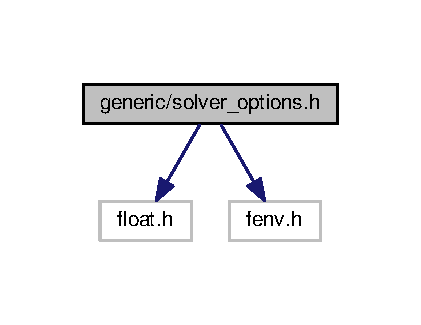
\includegraphics[width=186pt]{solver__options_8h__incl}
\end{center}
\end{figure}
This graph shows which files directly or indirectly include this file\+:
\nopagebreak
\begin{figure}[H]
\begin{center}
\leavevmode
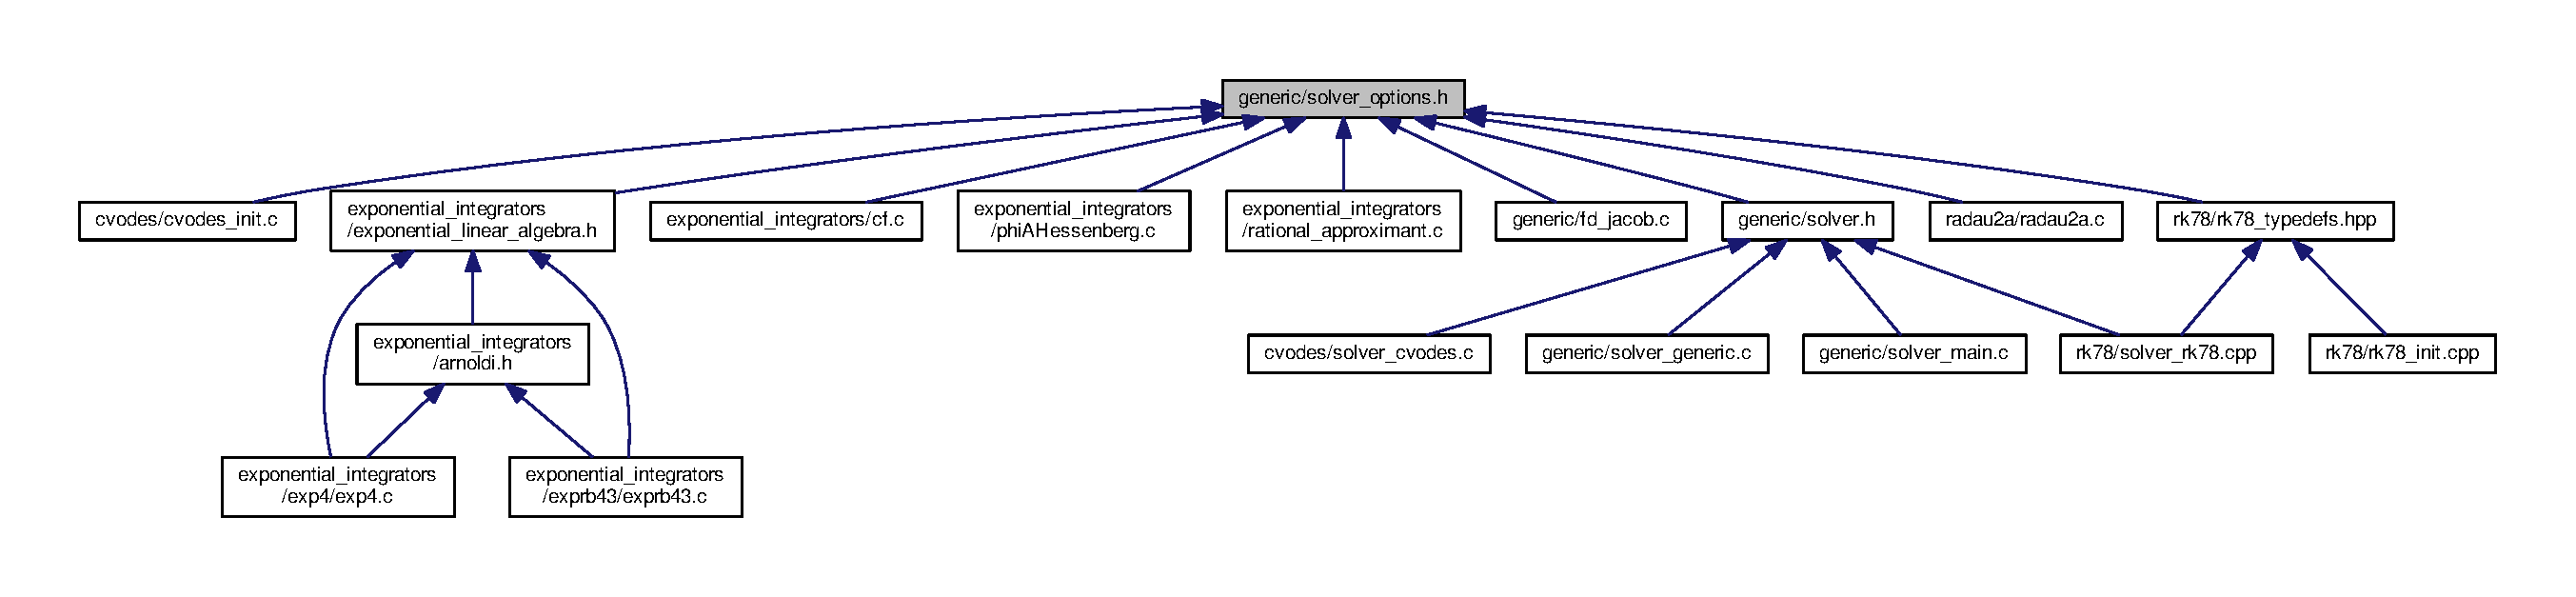
\includegraphics[width=350pt]{solver__options_8h__dep__incl}
\end{center}
\end{figure}
\subsection*{Macros}
\begin{DoxyCompactItemize}
\item 
\#define \hyperlink{solver__options_8h_a29a15cd00b37b1f4a5b4ec9f07c742f4}{A\+T\+OL}~(1e-\/10)
\item 
\#define \hyperlink{solver__options_8h_af50ac611d9fae906f9419504fd2caa5d}{R\+T\+OL}~(1e-\/06)
\item 
\#define \hyperlink{solver__options_8h_aaeb7127cf3bf0b49cec6554fbc101866}{t\+\_\+step}~(1e-\/06)
\item 
\#define \hyperlink{solver__options_8h_a25526ead9bdb589c90e7a8d3b4d1a746}{end\+\_\+time}~(1e-\/06)
\item 
\#define \hyperlink{solver__options_8h_a6ebf6899d6c1c8b7b9d09be872c05aae}{E\+PS}~D\+B\+L\+\_\+\+E\+P\+S\+I\+L\+ON
\item 
\#define \hyperlink{solver__options_8h_a09c78d2f8feb311dd9fc969a0bf84979}{S\+M\+A\+LL}~D\+B\+L\+\_\+\+M\+IN
\item 
\#define \hyperlink{solver__options_8h_a69f5533c684b73d07a7e20146a285cb1}{N\+\_\+\+RA}~(10)
\item 
\#define \hyperlink{solver__options_8h_a8dd330cbca99d70609ccc451d9099383}{C\+V\+\_\+\+M\+A\+X\+\_\+\+S\+T\+E\+PS}~(-\/1)
\item 
\#define \hyperlink{solver__options_8h_af45d9c410d5d7c99d2692080832d506e}{C\+V\+\_\+\+M\+A\+X\+\_\+\+H\+N\+IL}~(1)
\item 
\#define \hyperlink{solver__options_8h_ac42e0287ba619ab25b7d767a81f48082}{C\+V\+\_\+\+M\+A\+X\+\_\+\+E\+R\+R\+T\+E\+S\+T\+\_\+\+F\+A\+I\+LS}~(5)
\item 
\#define \hyperlink{solver__options_8h_aa98acf0dc83a3dce3ba168d75a74cb1b}{S\+A\+M\+E\+\_\+\+IC}
\item 
\#define \hyperlink{solver__options_8h_ad72dbcf6d0153db1b8d8a58001feed83}{D\+E\+B\+UG}
\item 
\#define \hyperlink{solver__options_8h_a0b43a0be2f674fea3218e7fb5221db1f}{S\+H\+U\+F\+F\+LE}
\item 
\#define \hyperlink{solver__options_8h_a8b43bafee90b30676faae508c21cb8d7}{P\+R\+I\+NT}
\item 
\#define \hyperlink{solver__options_8h_af5cccef89d39980a452b7f3a7c59fb53}{I\+GN}
\item 
\#define \hyperlink{solver__options_8h_ac786f5f1963363a48eed565f7cbc6931}{L\+O\+G\+\_\+\+O\+U\+T\+P\+UT}
\item 
\#define \hyperlink{solver__options_8h_a2adffa059bbd6f183ff7f63db602ac42}{L\+O\+G\+\_\+\+K\+R\+Y\+L\+O\+V\+\_\+\+A\+N\+D\+\_\+\+S\+T\+E\+P\+S\+I\+Z\+ES}
\item 
\#define \hyperlink{solver__options_8h_a09cc461392fae3949d88392adf655db5}{L\+O\+G\+\_\+\+E\+N\+D\+\_\+\+O\+N\+LY}
\item 
\#define \hyperlink{solver__options_8h_a9e28db46fb24c2d46dbfe205c6a11236}{F\+I\+N\+I\+T\+E\+\_\+\+D\+I\+F\+F\+E\+R\+E\+N\+CE}
\item 
\#define \hyperlink{solver__options_8h_a66c8290aad471b0be7768f635f03c349}{C\+O\+N\+S\+T\+\_\+\+T\+I\+M\+E\+\_\+\+S\+T\+EP}
\end{DoxyCompactItemize}


\subsection{Detailed Description}
A file generated by Scons that specifies various options to the solvers. 

This file, autogenerated by S\+Cons contains a number of definitions that can be enabled via command line options. These control the integrator behaviour and alternately enable special behaviour such as logging, divergence measuring, etc.

Note that it is not typical for all these options to be turned on at the same time, but it is done here for documentation purposes. 

\subsection{Macro Definition Documentation}
\index{solver\+\_\+options.\+h@{solver\+\_\+options.\+h}!A\+T\+OL@{A\+T\+OL}}
\index{A\+T\+OL@{A\+T\+OL}!solver\+\_\+options.\+h@{solver\+\_\+options.\+h}}
\subsubsection[{\texorpdfstring{A\+T\+OL}{ATOL}}]{\setlength{\rightskip}{0pt plus 5cm}\#define A\+T\+OL~(1e-\/10)}\hypertarget{solver__options_8h_a29a15cd00b37b1f4a5b4ec9f07c742f4}{}\label{solver__options_8h_a29a15cd00b37b1f4a5b4ec9f07c742f4}
Absolute solver tolerance \index{solver\+\_\+options.\+h@{solver\+\_\+options.\+h}!C\+O\+N\+S\+T\+\_\+\+T\+I\+M\+E\+\_\+\+S\+T\+EP@{C\+O\+N\+S\+T\+\_\+\+T\+I\+M\+E\+\_\+\+S\+T\+EP}}
\index{C\+O\+N\+S\+T\+\_\+\+T\+I\+M\+E\+\_\+\+S\+T\+EP@{C\+O\+N\+S\+T\+\_\+\+T\+I\+M\+E\+\_\+\+S\+T\+EP}!solver\+\_\+options.\+h@{solver\+\_\+options.\+h}}
\subsubsection[{\texorpdfstring{C\+O\+N\+S\+T\+\_\+\+T\+I\+M\+E\+\_\+\+S\+T\+EP}{CONST_TIME_STEP}}]{\setlength{\rightskip}{0pt plus 5cm}\#define C\+O\+N\+S\+T\+\_\+\+T\+I\+M\+E\+\_\+\+S\+T\+EP}\hypertarget{solver__options_8h_a66c8290aad471b0be7768f635f03c349}{}\label{solver__options_8h_a66c8290aad471b0be7768f635f03c349}
Define to turn off adaptive time stepping \index{solver\+\_\+options.\+h@{solver\+\_\+options.\+h}!C\+V\+\_\+\+M\+A\+X\+\_\+\+E\+R\+R\+T\+E\+S\+T\+\_\+\+F\+A\+I\+LS@{C\+V\+\_\+\+M\+A\+X\+\_\+\+E\+R\+R\+T\+E\+S\+T\+\_\+\+F\+A\+I\+LS}}
\index{C\+V\+\_\+\+M\+A\+X\+\_\+\+E\+R\+R\+T\+E\+S\+T\+\_\+\+F\+A\+I\+LS@{C\+V\+\_\+\+M\+A\+X\+\_\+\+E\+R\+R\+T\+E\+S\+T\+\_\+\+F\+A\+I\+LS}!solver\+\_\+options.\+h@{solver\+\_\+options.\+h}}
\subsubsection[{\texorpdfstring{C\+V\+\_\+\+M\+A\+X\+\_\+\+E\+R\+R\+T\+E\+S\+T\+\_\+\+F\+A\+I\+LS}{CV_MAX_ERRTEST_FAILS}}]{\setlength{\rightskip}{0pt plus 5cm}\#define C\+V\+\_\+\+M\+A\+X\+\_\+\+E\+R\+R\+T\+E\+S\+T\+\_\+\+F\+A\+I\+LS~(5)}\hypertarget{solver__options_8h_ac42e0287ba619ab25b7d767a81f48082}{}\label{solver__options_8h_ac42e0287ba619ab25b7d767a81f48082}
Maximum number of C\+V\+O\+DE error test fails before an error is thrown \index{solver\+\_\+options.\+h@{solver\+\_\+options.\+h}!C\+V\+\_\+\+M\+A\+X\+\_\+\+H\+N\+IL@{C\+V\+\_\+\+M\+A\+X\+\_\+\+H\+N\+IL}}
\index{C\+V\+\_\+\+M\+A\+X\+\_\+\+H\+N\+IL@{C\+V\+\_\+\+M\+A\+X\+\_\+\+H\+N\+IL}!solver\+\_\+options.\+h@{solver\+\_\+options.\+h}}
\subsubsection[{\texorpdfstring{C\+V\+\_\+\+M\+A\+X\+\_\+\+H\+N\+IL}{CV_MAX_HNIL}}]{\setlength{\rightskip}{0pt plus 5cm}\#define C\+V\+\_\+\+M\+A\+X\+\_\+\+H\+N\+IL~(1)}\hypertarget{solver__options_8h_af45d9c410d5d7c99d2692080832d506e}{}\label{solver__options_8h_af45d9c410d5d7c99d2692080832d506e}
Number of t + h == t warnings emitted by C\+V\+O\+DE (used to cleanup output) \index{solver\+\_\+options.\+h@{solver\+\_\+options.\+h}!C\+V\+\_\+\+M\+A\+X\+\_\+\+S\+T\+E\+PS@{C\+V\+\_\+\+M\+A\+X\+\_\+\+S\+T\+E\+PS}}
\index{C\+V\+\_\+\+M\+A\+X\+\_\+\+S\+T\+E\+PS@{C\+V\+\_\+\+M\+A\+X\+\_\+\+S\+T\+E\+PS}!solver\+\_\+options.\+h@{solver\+\_\+options.\+h}}
\subsubsection[{\texorpdfstring{C\+V\+\_\+\+M\+A\+X\+\_\+\+S\+T\+E\+PS}{CV_MAX_STEPS}}]{\setlength{\rightskip}{0pt plus 5cm}\#define C\+V\+\_\+\+M\+A\+X\+\_\+\+S\+T\+E\+PS~(-\/1)}\hypertarget{solver__options_8h_a8dd330cbca99d70609ccc451d9099383}{}\label{solver__options_8h_a8dd330cbca99d70609ccc451d9099383}
Maximum steps the solver will take in one timestep set to -\/1 (disabled) by default \index{solver\+\_\+options.\+h@{solver\+\_\+options.\+h}!D\+E\+B\+UG@{D\+E\+B\+UG}}
\index{D\+E\+B\+UG@{D\+E\+B\+UG}!solver\+\_\+options.\+h@{solver\+\_\+options.\+h}}
\subsubsection[{\texorpdfstring{D\+E\+B\+UG}{DEBUG}}]{\setlength{\rightskip}{0pt plus 5cm}\#define D\+E\+B\+UG}\hypertarget{solver__options_8h_ad72dbcf6d0153db1b8d8a58001feed83}{}\label{solver__options_8h_ad72dbcf6d0153db1b8d8a58001feed83}
Turn on debugging symbols, and use O0 optimization \index{solver\+\_\+options.\+h@{solver\+\_\+options.\+h}!end\+\_\+time@{end\+\_\+time}}
\index{end\+\_\+time@{end\+\_\+time}!solver\+\_\+options.\+h@{solver\+\_\+options.\+h}}
\subsubsection[{\texorpdfstring{end\+\_\+time}{end_time}}]{\setlength{\rightskip}{0pt plus 5cm}\#define end\+\_\+time~(1e-\/06)}\hypertarget{solver__options_8h_a25526ead9bdb589c90e7a8d3b4d1a746}{}\label{solver__options_8h_a25526ead9bdb589c90e7a8d3b4d1a746}
Global integration timestep \index{solver\+\_\+options.\+h@{solver\+\_\+options.\+h}!E\+PS@{E\+PS}}
\index{E\+PS@{E\+PS}!solver\+\_\+options.\+h@{solver\+\_\+options.\+h}}
\subsubsection[{\texorpdfstring{E\+PS}{EPS}}]{\setlength{\rightskip}{0pt plus 5cm}\#define E\+PS~D\+B\+L\+\_\+\+E\+P\+S\+I\+L\+ON}\hypertarget{solver__options_8h_a6ebf6899d6c1c8b7b9d09be872c05aae}{}\label{solver__options_8h_a6ebf6899d6c1c8b7b9d09be872c05aae}
Machine precision constant. \index{solver\+\_\+options.\+h@{solver\+\_\+options.\+h}!F\+I\+N\+I\+T\+E\+\_\+\+D\+I\+F\+F\+E\+R\+E\+N\+CE@{F\+I\+N\+I\+T\+E\+\_\+\+D\+I\+F\+F\+E\+R\+E\+N\+CE}}
\index{F\+I\+N\+I\+T\+E\+\_\+\+D\+I\+F\+F\+E\+R\+E\+N\+CE@{F\+I\+N\+I\+T\+E\+\_\+\+D\+I\+F\+F\+E\+R\+E\+N\+CE}!solver\+\_\+options.\+h@{solver\+\_\+options.\+h}}
\subsubsection[{\texorpdfstring{F\+I\+N\+I\+T\+E\+\_\+\+D\+I\+F\+F\+E\+R\+E\+N\+CE}{FINITE_DIFFERENCE}}]{\setlength{\rightskip}{0pt plus 5cm}\#define F\+I\+N\+I\+T\+E\+\_\+\+D\+I\+F\+F\+E\+R\+E\+N\+CE}\hypertarget{solver__options_8h_a9e28db46fb24c2d46dbfe205c6a11236}{}\label{solver__options_8h_a9e28db46fb24c2d46dbfe205c6a11236}
Use a Finite Difference Jaobian \index{solver\+\_\+options.\+h@{solver\+\_\+options.\+h}!I\+GN@{I\+GN}}
\index{I\+GN@{I\+GN}!solver\+\_\+options.\+h@{solver\+\_\+options.\+h}}
\subsubsection[{\texorpdfstring{I\+GN}{IGN}}]{\setlength{\rightskip}{0pt plus 5cm}\#define I\+GN}\hypertarget{solver__options_8h_af5cccef89d39980a452b7f3a7c59fb53}{}\label{solver__options_8h_af5cccef89d39980a452b7f3a7c59fb53}
Output ignition time (determined by simple T0 + 400 criteria) \index{solver\+\_\+options.\+h@{solver\+\_\+options.\+h}!L\+O\+G\+\_\+\+E\+N\+D\+\_\+\+O\+N\+LY@{L\+O\+G\+\_\+\+E\+N\+D\+\_\+\+O\+N\+LY}}
\index{L\+O\+G\+\_\+\+E\+N\+D\+\_\+\+O\+N\+LY@{L\+O\+G\+\_\+\+E\+N\+D\+\_\+\+O\+N\+LY}!solver\+\_\+options.\+h@{solver\+\_\+options.\+h}}
\subsubsection[{\texorpdfstring{L\+O\+G\+\_\+\+E\+N\+D\+\_\+\+O\+N\+LY}{LOG_END_ONLY}}]{\setlength{\rightskip}{0pt plus 5cm}\#define L\+O\+G\+\_\+\+E\+N\+D\+\_\+\+O\+N\+LY}\hypertarget{solver__options_8h_a09cc461392fae3949d88392adf655db5}{}\label{solver__options_8h_a09cc461392fae3949d88392adf655db5}
Log output to binary file only on final timestep \index{solver\+\_\+options.\+h@{solver\+\_\+options.\+h}!L\+O\+G\+\_\+\+K\+R\+Y\+L\+O\+V\+\_\+\+A\+N\+D\+\_\+\+S\+T\+E\+P\+S\+I\+Z\+ES@{L\+O\+G\+\_\+\+K\+R\+Y\+L\+O\+V\+\_\+\+A\+N\+D\+\_\+\+S\+T\+E\+P\+S\+I\+Z\+ES}}
\index{L\+O\+G\+\_\+\+K\+R\+Y\+L\+O\+V\+\_\+\+A\+N\+D\+\_\+\+S\+T\+E\+P\+S\+I\+Z\+ES@{L\+O\+G\+\_\+\+K\+R\+Y\+L\+O\+V\+\_\+\+A\+N\+D\+\_\+\+S\+T\+E\+P\+S\+I\+Z\+ES}!solver\+\_\+options.\+h@{solver\+\_\+options.\+h}}
\subsubsection[{\texorpdfstring{L\+O\+G\+\_\+\+K\+R\+Y\+L\+O\+V\+\_\+\+A\+N\+D\+\_\+\+S\+T\+E\+P\+S\+I\+Z\+ES}{LOG_KRYLOV_AND_STEPSIZES}}]{\setlength{\rightskip}{0pt plus 5cm}\#define L\+O\+G\+\_\+\+K\+R\+Y\+L\+O\+V\+\_\+\+A\+N\+D\+\_\+\+S\+T\+E\+P\+S\+I\+Z\+ES}\hypertarget{solver__options_8h_a2adffa059bbd6f183ff7f63db602ac42}{}\label{solver__options_8h_a2adffa059bbd6f183ff7f63db602ac42}
Turn on to log the krylov space and step sizes \index{solver\+\_\+options.\+h@{solver\+\_\+options.\+h}!L\+O\+G\+\_\+\+O\+U\+T\+P\+UT@{L\+O\+G\+\_\+\+O\+U\+T\+P\+UT}}
\index{L\+O\+G\+\_\+\+O\+U\+T\+P\+UT@{L\+O\+G\+\_\+\+O\+U\+T\+P\+UT}!solver\+\_\+options.\+h@{solver\+\_\+options.\+h}}
\subsubsection[{\texorpdfstring{L\+O\+G\+\_\+\+O\+U\+T\+P\+UT}{LOG_OUTPUT}}]{\setlength{\rightskip}{0pt plus 5cm}\#define L\+O\+G\+\_\+\+O\+U\+T\+P\+UT}\hypertarget{solver__options_8h_ac786f5f1963363a48eed565f7cbc6931}{}\label{solver__options_8h_ac786f5f1963363a48eed565f7cbc6931}
Log output to binary file \index{solver\+\_\+options.\+h@{solver\+\_\+options.\+h}!N\+\_\+\+RA@{N\+\_\+\+RA}}
\index{N\+\_\+\+RA@{N\+\_\+\+RA}!solver\+\_\+options.\+h@{solver\+\_\+options.\+h}}
\subsubsection[{\texorpdfstring{N\+\_\+\+RA}{N_RA}}]{\setlength{\rightskip}{0pt plus 5cm}\#define N\+\_\+\+RA~(10)}\hypertarget{solver__options_8h_a69f5533c684b73d07a7e20146a285cb1}{}\label{solver__options_8h_a69f5533c684b73d07a7e20146a285cb1}
type of rational approximant (n, n) \index{solver\+\_\+options.\+h@{solver\+\_\+options.\+h}!P\+R\+I\+NT@{P\+R\+I\+NT}}
\index{P\+R\+I\+NT@{P\+R\+I\+NT}!solver\+\_\+options.\+h@{solver\+\_\+options.\+h}}
\subsubsection[{\texorpdfstring{P\+R\+I\+NT}{PRINT}}]{\setlength{\rightskip}{0pt plus 5cm}\#define P\+R\+I\+NT}\hypertarget{solver__options_8h_a8b43bafee90b30676faae508c21cb8d7}{}\label{solver__options_8h_a8b43bafee90b30676faae508c21cb8d7}
Print the output to screen \index{solver\+\_\+options.\+h@{solver\+\_\+options.\+h}!R\+T\+OL@{R\+T\+OL}}
\index{R\+T\+OL@{R\+T\+OL}!solver\+\_\+options.\+h@{solver\+\_\+options.\+h}}
\subsubsection[{\texorpdfstring{R\+T\+OL}{RTOL}}]{\setlength{\rightskip}{0pt plus 5cm}\#define R\+T\+OL~(1e-\/06)}\hypertarget{solver__options_8h_af50ac611d9fae906f9419504fd2caa5d}{}\label{solver__options_8h_af50ac611d9fae906f9419504fd2caa5d}
Relative solver tolerance \index{solver\+\_\+options.\+h@{solver\+\_\+options.\+h}!S\+A\+M\+E\+\_\+\+IC@{S\+A\+M\+E\+\_\+\+IC}}
\index{S\+A\+M\+E\+\_\+\+IC@{S\+A\+M\+E\+\_\+\+IC}!solver\+\_\+options.\+h@{solver\+\_\+options.\+h}}
\subsubsection[{\texorpdfstring{S\+A\+M\+E\+\_\+\+IC}{SAME_IC}}]{\setlength{\rightskip}{0pt plus 5cm}\#define S\+A\+M\+E\+\_\+\+IC}\hypertarget{solver__options_8h_aa98acf0dc83a3dce3ba168d75a74cb1b}{}\label{solver__options_8h_aa98acf0dc83a3dce3ba168d75a74cb1b}
Load same initial conditions (defined in mechanism.\+c or mechanism.\+cu) for all threads \index{solver\+\_\+options.\+h@{solver\+\_\+options.\+h}!S\+H\+U\+F\+F\+LE@{S\+H\+U\+F\+F\+LE}}
\index{S\+H\+U\+F\+F\+LE@{S\+H\+U\+F\+F\+LE}!solver\+\_\+options.\+h@{solver\+\_\+options.\+h}}
\subsubsection[{\texorpdfstring{S\+H\+U\+F\+F\+LE}{SHUFFLE}}]{\setlength{\rightskip}{0pt plus 5cm}\#define S\+H\+U\+F\+F\+LE}\hypertarget{solver__options_8h_a0b43a0be2f674fea3218e7fb5221db1f}{}\label{solver__options_8h_a0b43a0be2f674fea3218e7fb5221db1f}
Use shuffled initial conditions \index{solver\+\_\+options.\+h@{solver\+\_\+options.\+h}!S\+M\+A\+LL@{S\+M\+A\+LL}}
\index{S\+M\+A\+LL@{S\+M\+A\+LL}!solver\+\_\+options.\+h@{solver\+\_\+options.\+h}}
\subsubsection[{\texorpdfstring{S\+M\+A\+LL}{SMALL}}]{\setlength{\rightskip}{0pt plus 5cm}\#define S\+M\+A\+LL~D\+B\+L\+\_\+\+M\+IN}\hypertarget{solver__options_8h_a09c78d2f8feb311dd9fc969a0bf84979}{}\label{solver__options_8h_a09c78d2f8feb311dd9fc969a0bf84979}
Smallest representable double \index{solver\+\_\+options.\+h@{solver\+\_\+options.\+h}!t\+\_\+step@{t\+\_\+step}}
\index{t\+\_\+step@{t\+\_\+step}!solver\+\_\+options.\+h@{solver\+\_\+options.\+h}}
\subsubsection[{\texorpdfstring{t\+\_\+step}{t_step}}]{\setlength{\rightskip}{0pt plus 5cm}\#define t\+\_\+step~(1e-\/06)}\hypertarget{solver__options_8h_aaeb7127cf3bf0b49cec6554fbc101866}{}\label{solver__options_8h_aaeb7127cf3bf0b49cec6554fbc101866}
Solver timestep (may be used to force multiple timesteps per global integration step) 
\hypertarget{radau2a_8c}{}\section{radau2a/radau2a.c File Reference}
\label{radau2a_8c}\index{radau2a/radau2a.\+c@{radau2a/radau2a.\+c}}
{\ttfamily \#include \char`\"{}header.\+h\char`\"{}}\\*
{\ttfamily \#include \char`\"{}solver\+\_\+props.\+h\char`\"{}}\\*
{\ttfamily \#include \char`\"{}solver\+\_\+options.\+h\char`\"{}}\\*
{\ttfamily \#include \char`\"{}lapack\+\_\+dfns.\+h\char`\"{}}\\*
{\ttfamily \#include \char`\"{}dydt.\+h\char`\"{}}\\*
{\ttfamily \#include \char`\"{}jacob.\+h\char`\"{}}\\*
{\ttfamily \#include $<$complex.\+h$>$}\\*
{\ttfamily \#include $<$stdio.\+h$>$}\\*
{\ttfamily \#include $<$stdbool.\+h$>$}\\*
{\ttfamily \#include $<$string.\+h$>$}\\*
Include dependency graph for radau2a.\+c\+:
\nopagebreak
\begin{figure}[H]
\begin{center}
\leavevmode
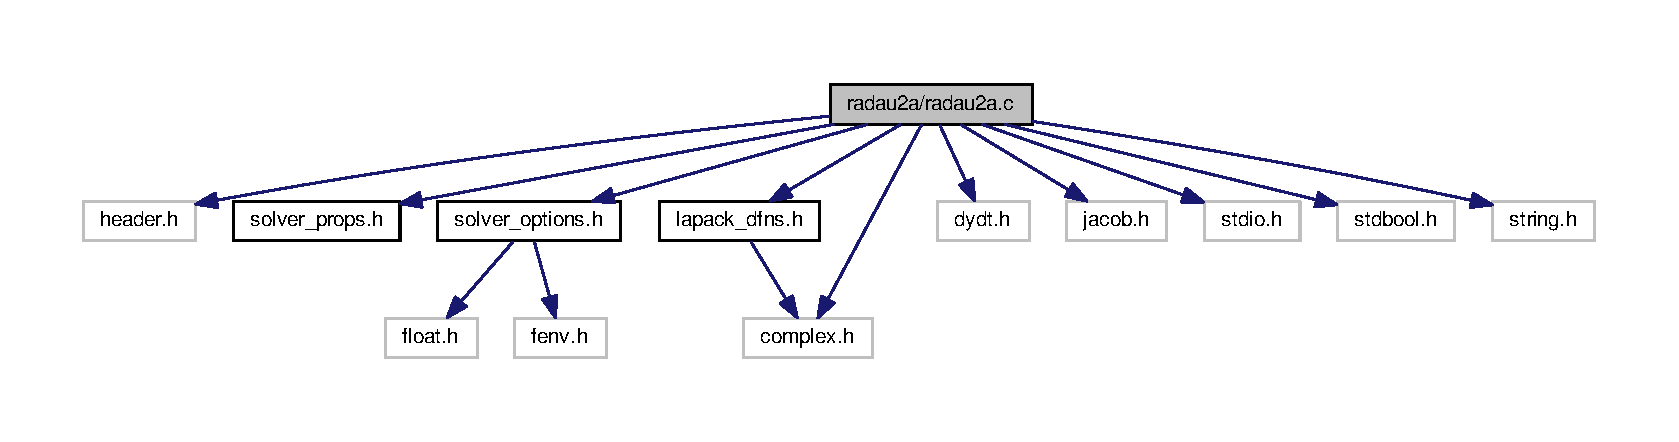
\includegraphics[width=350pt]{radau2a_8c__incl}
\end{center}
\end{figure}
\subsection*{Macros}
\begin{DoxyCompactItemize}
\item 
\#define {\bfseries Max\+\_\+no\+\_\+steps}~(200000)\hypertarget{radau2a_8c_a4f5652e996f678da1b1b93c8aa4a7961}{}\label{radau2a_8c_a4f5652e996f678da1b1b93c8aa4a7961}

\item 
\#define {\bfseries Newton\+Maxit}~(8)\hypertarget{radau2a_8c_ab408861ee5149b85ac129cb8a3875743}{}\label{radau2a_8c_ab408861ee5149b85ac129cb8a3875743}

\item 
\#define {\bfseries Start\+Newton}~(true)\hypertarget{radau2a_8c_aa9c48bc3c2002ed4e6792dd7f526d783}{}\label{radau2a_8c_aa9c48bc3c2002ed4e6792dd7f526d783}

\item 
\#define {\bfseries Gustafsson}\hypertarget{radau2a_8c_a619cdc11d911799dd674458eb84dc349}{}\label{radau2a_8c_a619cdc11d911799dd674458eb84dc349}

\item 
\#define {\bfseries Roundoff}~(\hyperlink{solver__options_8h_a6ebf6899d6c1c8b7b9d09be872c05aae}{E\+PS})\hypertarget{radau2a_8c_a0628e9521e9961c49b173765f9d815d3}{}\label{radau2a_8c_a0628e9521e9961c49b173765f9d815d3}

\item 
\#define {\bfseries Fac\+Min}~(0.\+2)\hypertarget{radau2a_8c_a2709085ffea146cba50846d860f7d945}{}\label{radau2a_8c_a2709085ffea146cba50846d860f7d945}

\item 
\#define {\bfseries Fac\+Max}~(8)\hypertarget{radau2a_8c_a3ae724566d10e7ae2a48e1d340d6937b}{}\label{radau2a_8c_a3ae724566d10e7ae2a48e1d340d6937b}

\item 
\#define {\bfseries Fac\+Safe}~(0.\+9)\hypertarget{radau2a_8c_a29559e0d6fcf09d76688dbc471b01219}{}\label{radau2a_8c_a29559e0d6fcf09d76688dbc471b01219}

\item 
\#define {\bfseries Fac\+Rej}~(0.\+1)\hypertarget{radau2a_8c_afb5b5659c29086c78a546a078c08238f}{}\label{radau2a_8c_afb5b5659c29086c78a546a078c08238f}

\item 
\#define {\bfseries Theta\+Min}~(0.\+001)\hypertarget{radau2a_8c_a1dea03e748069283de9d62ca81b64e75}{}\label{radau2a_8c_a1dea03e748069283de9d62ca81b64e75}

\item 
\#define {\bfseries Newton\+Tol}~(0.\+03)\hypertarget{radau2a_8c_a5ea658585341bf26e79bbf1ed3497e6f}{}\label{radau2a_8c_a5ea658585341bf26e79bbf1ed3497e6f}

\item 
\#define {\bfseries Qmin}~(1.\+0)\hypertarget{radau2a_8c_ac523cd36edc6fc54a93dfdb10a772bc0}{}\label{radau2a_8c_ac523cd36edc6fc54a93dfdb10a772bc0}

\item 
\#define {\bfseries Qmax}~(1.\+2)\hypertarget{radau2a_8c_afcfd11ffcebe8a32d20dcacebefa7e6f}{}\label{radau2a_8c_afcfd11ffcebe8a32d20dcacebefa7e6f}

\item 
\#define {\bfseries U\+N\+R\+O\+LL}~(8)\hypertarget{radau2a_8c_a870020ccb79b9bf241010e975e029bde}{}\label{radau2a_8c_a870020ccb79b9bf241010e975e029bde}

\end{DoxyCompactItemize}
\subsection*{Functions}
\begin{DoxyCompactItemize}
\item 
int \hyperlink{radau2a_8c_a01c536019d80bd2cbfe04acfa0c68db1}{integrate} (const double t\+\_\+start, const double t\+\_\+end, const double pr, double $\ast$y)
\end{DoxyCompactItemize}


\subsection{Detailed Description}
\begin{DoxyAuthor}{Author}
Nicholas J. Curtis 
\end{DoxyAuthor}
\begin{DoxyDate}{Date}
03/16/2015
\end{DoxyDate}
A Radau2A I\+RK implementation for C

N\+O\+TE\+: all matricies stored in column major format! 

\subsection{Function Documentation}
\index{radau2a.\+c@{radau2a.\+c}!integrate@{integrate}}
\index{integrate@{integrate}!radau2a.\+c@{radau2a.\+c}}
\subsubsection[{\texorpdfstring{integrate(const double t\+\_\+start, const double t\+\_\+end, const double pr, double $\ast$y)}{integrate(const double t_start, const double t_end, const double pr, double *y)}}]{\setlength{\rightskip}{0pt plus 5cm}int integrate (
\begin{DoxyParamCaption}
\item[{const double}]{t\+\_\+start, }
\item[{const double}]{t\+\_\+end, }
\item[{const double}]{pr, }
\item[{double $\ast$}]{y}
\end{DoxyParamCaption}
)}\hypertarget{radau2a_8c_a01c536019d80bd2cbfe04acfa0c68db1}{}\label{radau2a_8c_a01c536019d80bd2cbfe04acfa0c68db1}
5th-\/order Radau2A implementation Non-\/convergence of Newton\+: Theta too large

$\sim$$\sim$$\sim$$>$ Computation of new step size Hnew 
\hypertarget{radau2a_8cu}{}\section{radau2a/radau2a.cu File Reference}
\label{radau2a_8cu}\index{radau2a/radau2a.\+cu@{radau2a/radau2a.\+cu}}


A Radau2A I\+RK implementation for C\+U\+DA Adapted from Hairer and Wanner\textquotesingle{}s \href{http://www.unige.ch/~hairer/prog/stiff/radau5.f}{\tt R\+A\+D\+A\+U5 code} and the \href{http://people.cs.vt.edu/~asandu/Software/FATODE/index.html}{\tt F\+A\+T\+O\+DE} O\+DE integration library.  


{\ttfamily \#include $<$cu\+Complex.\+h$>$}\\*
{\ttfamily \#include \char`\"{}header.\+cuh\char`\"{}}\\*
{\ttfamily \#include \char`\"{}solver\+\_\+options.\+cuh\char`\"{}}\\*
{\ttfamily \#include \char`\"{}solver\+\_\+props.\+cuh\char`\"{}}\\*
{\ttfamily \#include \char`\"{}inverse.\+cuh\char`\"{}}\\*
{\ttfamily \#include \char`\"{}complex\+Inverse.\+cuh\char`\"{}}\\*
{\ttfamily \#include \char`\"{}jacob.\+cuh\char`\"{}}\\*
{\ttfamily \#include \char`\"{}dydt.\+cuh\char`\"{}}\\*
{\ttfamily \#include \char`\"{}gpu\+\_\+macros.\+cuh\char`\"{}}\\*
Include dependency graph for radau2a.\+cu\+:\nopagebreak
\begin{figure}[H]
\begin{center}
\leavevmode
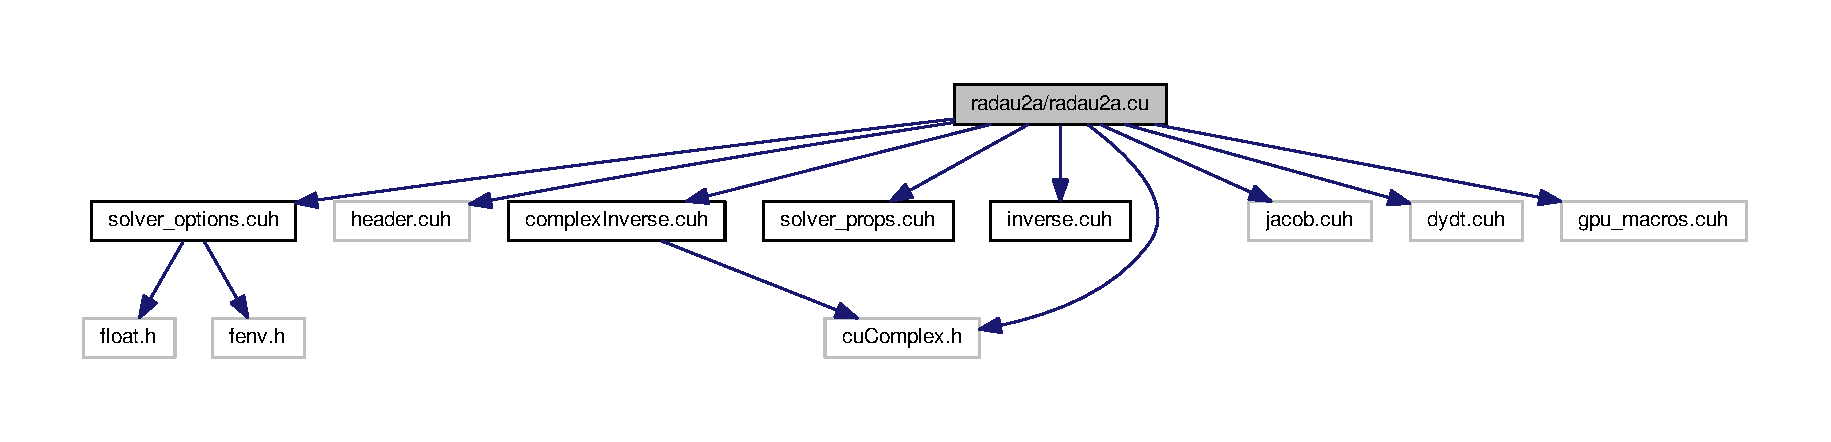
\includegraphics[width=350pt]{radau2a_8cu__incl}
\end{center}
\end{figure}
\subsection*{Macros}
\begin{DoxyCompactItemize}
\item 
\#define \hyperlink{radau2a_8cu_a1fb079c51babe820cd76885d3c519446}{A\+NY}(X)~((X))
\item 
\#define \hyperlink{radau2a_8cu_ada568356af1dada57942e4b6e5d271b0}{A\+LL}(X)~((X))
\item 
\#define \hyperlink{radau2a_8cu_a4f5652e996f678da1b1b93c8aa4a7961}{Max\+\_\+no\+\_\+steps}~(200000)
\item 
\#define \hyperlink{radau2a_8cu_ab408861ee5149b85ac129cb8a3875743}{Newton\+Maxit}~(8)
\item 
\#define \hyperlink{radau2a_8cu_aa9c48bc3c2002ed4e6792dd7f526d783}{Start\+Newton}~(true)
\item 
\#define \hyperlink{radau2a_8cu_a619cdc11d911799dd674458eb84dc349}{Gustafsson}
\item 
\#define \hyperlink{radau2a_8cu_a0628e9521e9961c49b173765f9d815d3}{Roundoff}~(\hyperlink{solver__options_8h_a6ebf6899d6c1c8b7b9d09be872c05aae}{E\+PS})
\item 
\#define \hyperlink{radau2a_8cu_a2709085ffea146cba50846d860f7d945}{Fac\+Min}~(0.\+2)
\item 
\#define \hyperlink{radau2a_8cu_a3ae724566d10e7ae2a48e1d340d6937b}{Fac\+Max}~(8)
\item 
\#define \hyperlink{radau2a_8cu_a29559e0d6fcf09d76688dbc471b01219}{Fac\+Safe}~(0.\+9)
\item 
\#define \hyperlink{radau2a_8cu_afb5b5659c29086c78a546a078c08238f}{Fac\+Rej}~(0.\+1)
\item 
\#define \hyperlink{radau2a_8cu_a1dea03e748069283de9d62ca81b64e75}{Theta\+Min}~(0.\+001)
\item 
\#define \hyperlink{radau2a_8cu_a5ea658585341bf26e79bbf1ed3497e6f}{Newton\+Tol}~(0.\+03)
\item 
\#define \hyperlink{radau2a_8cu_ac523cd36edc6fc54a93dfdb10a772bc0}{Qmin}~(1.\+0)
\item 
\#define \hyperlink{radau2a_8cu_afcfd11ffcebe8a32d20dcacebefa7e6f}{Qmax}~(1.\+2)
\item 
\#define \hyperlink{radau2a_8cu_a172b5bc0830959ab49ca7cb9f0ae44bf}{Max\+\_\+consecutive\+\_\+errs}~(5)
\end{DoxyCompactItemize}


\subsection{Detailed Description}
A Radau2A I\+RK implementation for C\+U\+DA Adapted from Hairer and Wanner\textquotesingle{}s \href{http://www.unige.ch/~hairer/prog/stiff/radau5.f}{\tt R\+A\+D\+A\+U5 code} and the \href{http://people.cs.vt.edu/~asandu/Software/FATODE/index.html}{\tt F\+A\+T\+O\+DE} O\+DE integration library. 

\begin{DoxyAuthor}{Author}
Nicholas J. Curtis 
\end{DoxyAuthor}
\begin{DoxyDate}{Date}
03/16/2015
\end{DoxyDate}
For full reference see\+:~\newline
 G. Wanner, E. Hairer, Solving Ordinary Differential Equations II\+: Stiff and Differential\+Algebraic Problems, 2nd Edition, Springer-\/\+Verlag, Berlin, 1996. doi\+:10.\+1007/978-\/3-\/642-\/ 05221-\/7.

N\+O\+TE\+: all matricies stored in column major format! 

\subsection{Macro Definition Documentation}
\index{radau2a.\+cu@{radau2a.\+cu}!A\+LL@{A\+LL}}
\index{A\+LL@{A\+LL}!radau2a.\+cu@{radau2a.\+cu}}
\subsubsection[{\texorpdfstring{A\+LL}{ALL}}]{\setlength{\rightskip}{0pt plus 5cm}\#define A\+LL(
\begin{DoxyParamCaption}
\item[{}]{X}
\end{DoxyParamCaption}
)~((X))}\hypertarget{radau2a_8cu_ada568356af1dada57942e4b6e5d271b0}{}\label{radau2a_8cu_ada568356af1dada57942e4b6e5d271b0}
\index{radau2a.\+cu@{radau2a.\+cu}!A\+NY@{A\+NY}}
\index{A\+NY@{A\+NY}!radau2a.\+cu@{radau2a.\+cu}}
\subsubsection[{\texorpdfstring{A\+NY}{ANY}}]{\setlength{\rightskip}{0pt plus 5cm}\#define A\+NY(
\begin{DoxyParamCaption}
\item[{}]{X}
\end{DoxyParamCaption}
)~((X))}\hypertarget{radau2a_8cu_a1fb079c51babe820cd76885d3c519446}{}\label{radau2a_8cu_a1fb079c51babe820cd76885d3c519446}
\index{radau2a.\+cu@{radau2a.\+cu}!Fac\+Max@{Fac\+Max}}
\index{Fac\+Max@{Fac\+Max}!radau2a.\+cu@{radau2a.\+cu}}
\subsubsection[{\texorpdfstring{Fac\+Max}{FacMax}}]{\setlength{\rightskip}{0pt plus 5cm}\#define Fac\+Max~(8)}\hypertarget{radau2a_8cu_a3ae724566d10e7ae2a48e1d340d6937b}{}\label{radau2a_8cu_a3ae724566d10e7ae2a48e1d340d6937b}
\index{radau2a.\+cu@{radau2a.\+cu}!Fac\+Min@{Fac\+Min}}
\index{Fac\+Min@{Fac\+Min}!radau2a.\+cu@{radau2a.\+cu}}
\subsubsection[{\texorpdfstring{Fac\+Min}{FacMin}}]{\setlength{\rightskip}{0pt plus 5cm}\#define Fac\+Min~(0.\+2)}\hypertarget{radau2a_8cu_a2709085ffea146cba50846d860f7d945}{}\label{radau2a_8cu_a2709085ffea146cba50846d860f7d945}
\index{radau2a.\+cu@{radau2a.\+cu}!Fac\+Rej@{Fac\+Rej}}
\index{Fac\+Rej@{Fac\+Rej}!radau2a.\+cu@{radau2a.\+cu}}
\subsubsection[{\texorpdfstring{Fac\+Rej}{FacRej}}]{\setlength{\rightskip}{0pt plus 5cm}\#define Fac\+Rej~(0.\+1)}\hypertarget{radau2a_8cu_afb5b5659c29086c78a546a078c08238f}{}\label{radau2a_8cu_afb5b5659c29086c78a546a078c08238f}
\index{radau2a.\+cu@{radau2a.\+cu}!Fac\+Safe@{Fac\+Safe}}
\index{Fac\+Safe@{Fac\+Safe}!radau2a.\+cu@{radau2a.\+cu}}
\subsubsection[{\texorpdfstring{Fac\+Safe}{FacSafe}}]{\setlength{\rightskip}{0pt plus 5cm}\#define Fac\+Safe~(0.\+9)}\hypertarget{radau2a_8cu_a29559e0d6fcf09d76688dbc471b01219}{}\label{radau2a_8cu_a29559e0d6fcf09d76688dbc471b01219}
\index{radau2a.\+cu@{radau2a.\+cu}!Gustafsson@{Gustafsson}}
\index{Gustafsson@{Gustafsson}!radau2a.\+cu@{radau2a.\+cu}}
\subsubsection[{\texorpdfstring{Gustafsson}{Gustafsson}}]{\setlength{\rightskip}{0pt plus 5cm}\#define Gustafsson}\hypertarget{radau2a_8cu_a619cdc11d911799dd674458eb84dc349}{}\label{radau2a_8cu_a619cdc11d911799dd674458eb84dc349}
\index{radau2a.\+cu@{radau2a.\+cu}!Max\+\_\+consecutive\+\_\+errs@{Max\+\_\+consecutive\+\_\+errs}}
\index{Max\+\_\+consecutive\+\_\+errs@{Max\+\_\+consecutive\+\_\+errs}!radau2a.\+cu@{radau2a.\+cu}}
\subsubsection[{\texorpdfstring{Max\+\_\+consecutive\+\_\+errs}{Max_consecutive_errs}}]{\setlength{\rightskip}{0pt plus 5cm}\#define Max\+\_\+consecutive\+\_\+errs~(5)}\hypertarget{radau2a_8cu_a172b5bc0830959ab49ca7cb9f0ae44bf}{}\label{radau2a_8cu_a172b5bc0830959ab49ca7cb9f0ae44bf}
\index{radau2a.\+cu@{radau2a.\+cu}!Max\+\_\+no\+\_\+steps@{Max\+\_\+no\+\_\+steps}}
\index{Max\+\_\+no\+\_\+steps@{Max\+\_\+no\+\_\+steps}!radau2a.\+cu@{radau2a.\+cu}}
\subsubsection[{\texorpdfstring{Max\+\_\+no\+\_\+steps}{Max_no_steps}}]{\setlength{\rightskip}{0pt plus 5cm}\#define Max\+\_\+no\+\_\+steps~(200000)}\hypertarget{radau2a_8cu_a4f5652e996f678da1b1b93c8aa4a7961}{}\label{radau2a_8cu_a4f5652e996f678da1b1b93c8aa4a7961}
\index{radau2a.\+cu@{radau2a.\+cu}!Newton\+Maxit@{Newton\+Maxit}}
\index{Newton\+Maxit@{Newton\+Maxit}!radau2a.\+cu@{radau2a.\+cu}}
\subsubsection[{\texorpdfstring{Newton\+Maxit}{NewtonMaxit}}]{\setlength{\rightskip}{0pt plus 5cm}\#define Newton\+Maxit~(8)}\hypertarget{radau2a_8cu_ab408861ee5149b85ac129cb8a3875743}{}\label{radau2a_8cu_ab408861ee5149b85ac129cb8a3875743}
\index{radau2a.\+cu@{radau2a.\+cu}!Newton\+Tol@{Newton\+Tol}}
\index{Newton\+Tol@{Newton\+Tol}!radau2a.\+cu@{radau2a.\+cu}}
\subsubsection[{\texorpdfstring{Newton\+Tol}{NewtonTol}}]{\setlength{\rightskip}{0pt plus 5cm}\#define Newton\+Tol~(0.\+03)}\hypertarget{radau2a_8cu_a5ea658585341bf26e79bbf1ed3497e6f}{}\label{radau2a_8cu_a5ea658585341bf26e79bbf1ed3497e6f}
\index{radau2a.\+cu@{radau2a.\+cu}!Qmax@{Qmax}}
\index{Qmax@{Qmax}!radau2a.\+cu@{radau2a.\+cu}}
\subsubsection[{\texorpdfstring{Qmax}{Qmax}}]{\setlength{\rightskip}{0pt plus 5cm}\#define Qmax~(1.\+2)}\hypertarget{radau2a_8cu_afcfd11ffcebe8a32d20dcacebefa7e6f}{}\label{radau2a_8cu_afcfd11ffcebe8a32d20dcacebefa7e6f}
\index{radau2a.\+cu@{radau2a.\+cu}!Qmin@{Qmin}}
\index{Qmin@{Qmin}!radau2a.\+cu@{radau2a.\+cu}}
\subsubsection[{\texorpdfstring{Qmin}{Qmin}}]{\setlength{\rightskip}{0pt plus 5cm}\#define Qmin~(1.\+0)}\hypertarget{radau2a_8cu_ac523cd36edc6fc54a93dfdb10a772bc0}{}\label{radau2a_8cu_ac523cd36edc6fc54a93dfdb10a772bc0}
\index{radau2a.\+cu@{radau2a.\+cu}!Roundoff@{Roundoff}}
\index{Roundoff@{Roundoff}!radau2a.\+cu@{radau2a.\+cu}}
\subsubsection[{\texorpdfstring{Roundoff}{Roundoff}}]{\setlength{\rightskip}{0pt plus 5cm}\#define Roundoff~({\bf E\+PS})}\hypertarget{radau2a_8cu_a0628e9521e9961c49b173765f9d815d3}{}\label{radau2a_8cu_a0628e9521e9961c49b173765f9d815d3}
\index{radau2a.\+cu@{radau2a.\+cu}!Start\+Newton@{Start\+Newton}}
\index{Start\+Newton@{Start\+Newton}!radau2a.\+cu@{radau2a.\+cu}}
\subsubsection[{\texorpdfstring{Start\+Newton}{StartNewton}}]{\setlength{\rightskip}{0pt plus 5cm}\#define Start\+Newton~(true)}\hypertarget{radau2a_8cu_aa9c48bc3c2002ed4e6792dd7f526d783}{}\label{radau2a_8cu_aa9c48bc3c2002ed4e6792dd7f526d783}
\index{radau2a.\+cu@{radau2a.\+cu}!Theta\+Min@{Theta\+Min}}
\index{Theta\+Min@{Theta\+Min}!radau2a.\+cu@{radau2a.\+cu}}
\subsubsection[{\texorpdfstring{Theta\+Min}{ThetaMin}}]{\setlength{\rightskip}{0pt plus 5cm}\#define Theta\+Min~(0.\+001)}\hypertarget{radau2a_8cu_a1dea03e748069283de9d62ca81b64e75}{}\label{radau2a_8cu_a1dea03e748069283de9d62ca81b64e75}

%--- End generated contents ---

% Index
\backmatter
\newpage
\phantomsection
\clearemptydoublepage
\addcontentsline{toc}{chapter}{Index}
\printindex

\end{document}
